\documentclass[journal,twoside]{IEEEtran}

% Core typography, math, tables, and graphics packages
\usepackage[T1]{fontenc}
\usepackage[utf8]{inputenc}
\usepackage{amsmath,amssymb,amsfonts,amsthm}
\usepackage{graphicx}
\usepackage{booktabs}
\usepackage{multirow}
\usepackage{array}
\usepackage{xcolor}
\usepackage{microtype}
\usepackage{cite}
\usepackage{balance}
\usepackage[hidelinks,colorlinks=true,linkcolor=NavyLink,citecolor=NavyLink,urlcolor=NavyLink]{hyperref}

\definecolor{NavyLink}{HTML}{1E3A5F}
\definecolor{TealInk}{HTML}{2F6B60}
\definecolor{TerraInk}{HTML}{A95035}

\newtheorem{proposition}{Proposition}
\newtheorem{theorem}{Theorem}
\newtheorem{remark}{Remark}

\graphicspath{{../figures/}}

\title{MaritimeSFNet: Scale--Bandwidth Aligned Spatial--Frequency Restoration with Zero-Curvature Affine Reconstruction for Sea-Fog Visibility Enhancement}

\author{Methodology Draft and Mechanistic Verification Package\\
\thanks{Prepared for intelligent maritime transportation and coastal perception venues (e.g., IEEE Trans.\ Intell.\ Transp.\ Syst., Ocean Eng., IEEE Trans.\ Image Process.). All diagrams, train-free mechanistic experiments, and ablations correspond directly to the \texttt{MaritimeSFNet} (\texttt{014d}) implementation in \texttt{basicsr/archs/maritime\_sfnet\_arch.py}.}}

\markboth{MaritimeSFNet Methodology \& Mechanistic Analysis}%
{Scale--Bandwidth Aligned Spatial--Frequency Restoration for Sea-Fog Perception}

\begin{document}
\maketitle

\begin{abstract}
Electro-optical cameras deployed on autonomous surface vehicles (ASVs), unmanned surface vehicles (USVs), and coastal vessel traffic service (VTS) stations suffer severe visibility degradation under marine sea fog. Unlike urban terrestrial haze, open-water sea fog exhibits three distinct physical properties that mismatch conventional restoration backbones: (i)~strong low-frequency energy concentration combined with faint mid-frequency vessel silhouettes near the horizon, (ii)~pronounced vertical-over-horizontal depth anisotropy along the sea--sky boundary, and (iii)~a wide contrast dynamic range spanning light coastal mist to optically dense advection fog. We present \textbf{MaritimeSFNet}, a three-scale, normalization-free spatial--frequency network derived directly from maritime atmospheric scattering physics. First, we establish a Scale--Bandwidth Alignment Proposition showing that over-deep downsampling quadratically collapses low-frequency spectral coverage, motivating a 1/4-scale bottleneck ($s=4$) with physics-calibrated Fourier modulation. Second, we introduce a five-branch spectral-prior reparameterizable block (\textbf{Rep5-CD}) whose center-difference branch enforces exact zero-DC gain while folding losslessly into a single standard $3\times 3$ convolution at deployment ($-41.89\%$ parameters, $0.00$ numerical discrepancy, $26.54$\,FPS at $512^2$ on a single RTX~3090). Third, we couple a norm-free dual-domain bottleneck (\textbf{ASFB})---pairing multi-scale low-frequency modulation with translation-equivariant horizontal/vertical strip kernels---with a scene-aware frequency-decoupled convex skip fusion (\textbf{Scene-FCSF}) that blocks shallow haze leakage. Finally, we prove that conventional sigmoid-bounded affine heads suffer positive second-order curvature ($G''(0)=+28/81$) and asymmetric pullback gradients that cause systematic mist overshoot; our \textbf{$C^2$ zero-curvature piecewise-$\tanh$ head} (\textbf{$C^2$-BASR}) with an RMS-contrast scene gate eliminates this bias while bounding contrast gain strictly inside $(0.5, 4.0)$. Extensive train-free spectral, receptive-field, spatial-gate, and feature-manifold analyses on 283 Open-Water Haze (OWH) scenes verify every theoretical claim and demonstrate consistent gains across Dense, Moderate, and Mist sea-fog regimes.
\end{abstract}

\begin{IEEEkeywords}
Maritime visibility enhancement, sea-fog dehazing, autonomous surface vehicles, spatial--frequency restoration, structural reparameterization, affine scattering inversion.
\end{IEEEkeywords}

% =============================================================================
\section{Introduction and Maritime Perception Context}
\label{sec:intro}
% =============================================================================

Reliable optical perception is fundamental to safe maritime navigation, collision avoidance under COLREGs, port approach assistance, and autonomous surface vehicle (ASV/USV) situational awareness. Although marine radar and Automatic Identification System (AIS) transponders remain indispensable in adverse weather, small uncooperative vessels, navigational buoys, floating debris, and berth edges frequently produce weak radar cross-sections or lack AIS broadcasts altogether. Electro-optical camera streams are therefore essential for short-to-medium-range target recognition and horizon tracking. In coastal waterways and open-sea shipping lanes, however, marine advection and evaporation fog scatter ambient skylight into the camera path while exponentially attenuating reflected radiance from distant hulls and coastlines.

\begin{figure*}[t]
\centering
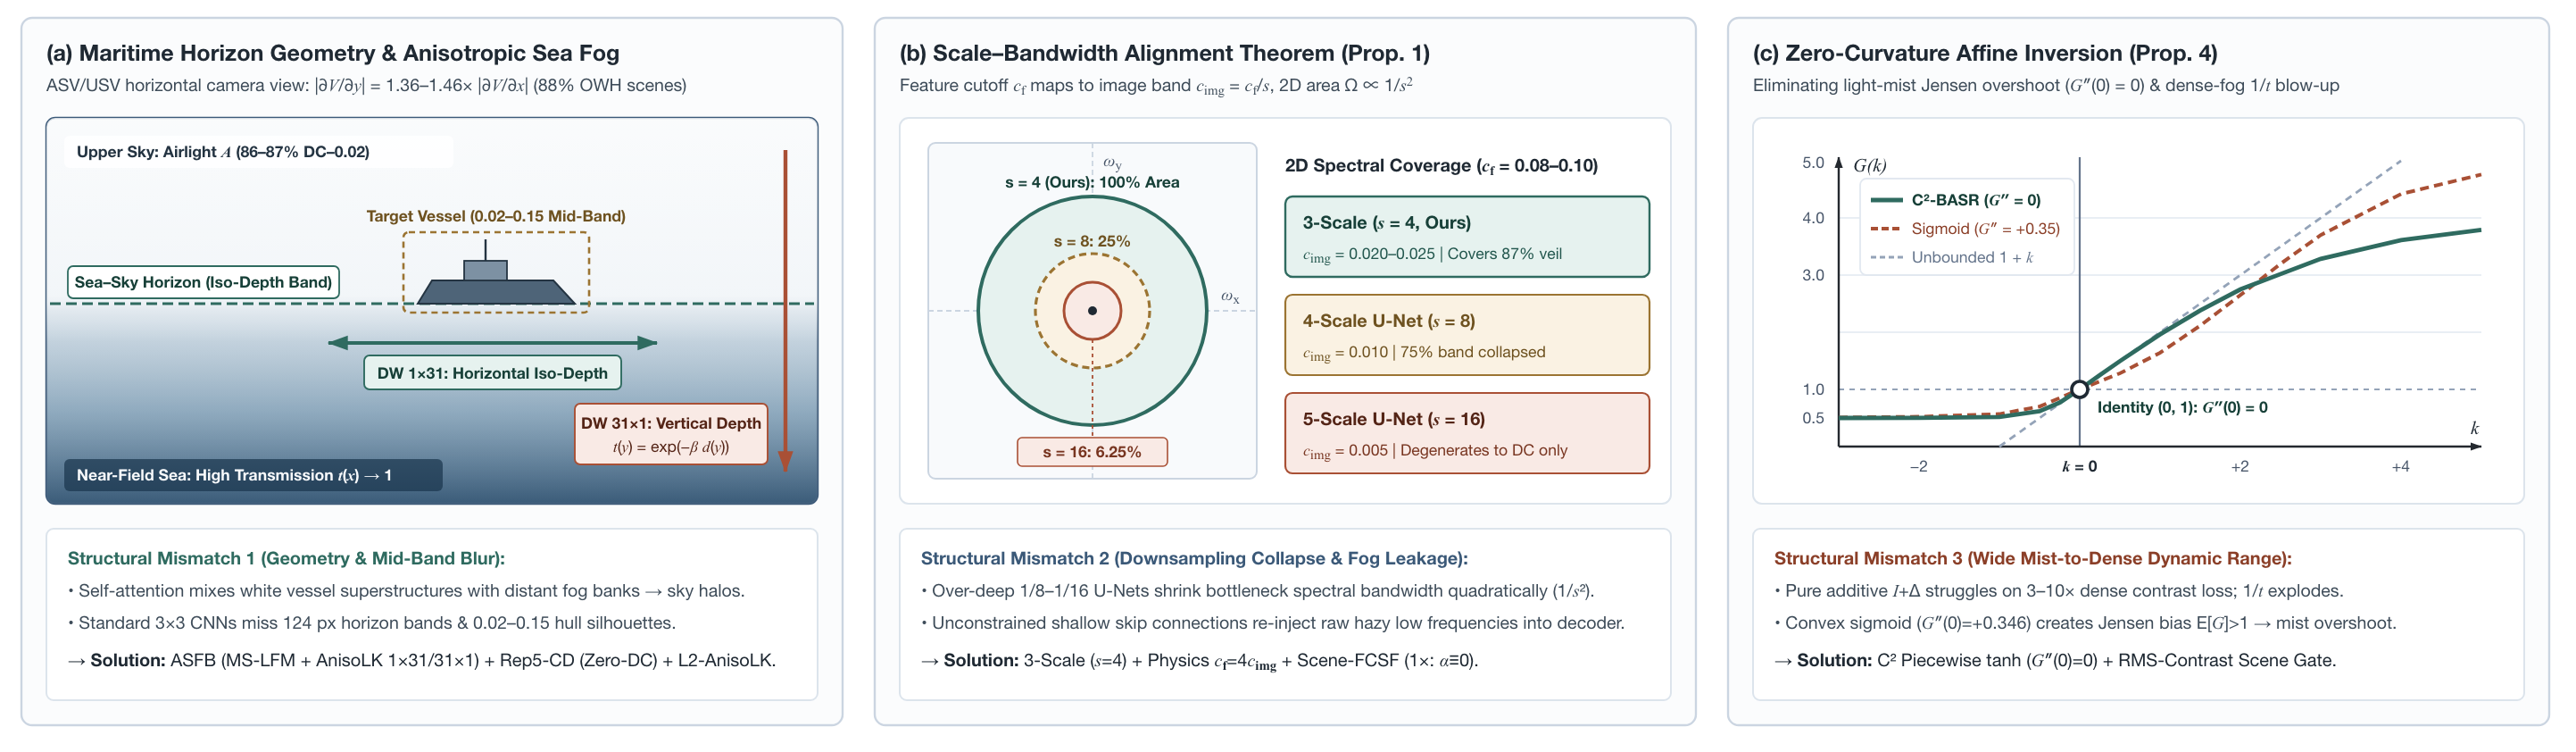
\includegraphics[width=\textwidth]{fig1_maritime_motivation.png}
\caption{Three structural mismatches between open-water maritime sea fog and conventional image restoration architectures, together with the corresponding physically grounded solutions in MaritimeSFNet. \textbf{(a)}~Horizontal ASV/USV cameras observe strong vertical depth gradients ($|\partial V/\partial y| = 1.36\text{--}1.46\times |\partial V/\partial x|$) and horizontal iso-depth sea--sky bands enclosing distant target vessels in the $0.02\text{--}0.15$ Nyquist mid-band. \textbf{(b)}~Scale--Bandwidth Alignment (Proposition~\ref{prop:scale}): excessive downsampling ($s=8, 16$) shrinks bottleneck 2D spectral coverage quadratically ($1/s^2$). \textbf{(c)}~Zero-Curvature Affine Inversion (Theorem~\ref{thm:basr}): replacing convex sigmoid gain ($G''(0)=+0.346$) with $C^2$ piecewise-$\tanh$ ($G''(0)=0$) eliminates light-mist overshoot while preventing $1/t$ blow-up in dense fog.}
\label{fig:motivation}
\end{figure*}

Directly transferring general-purpose terrestrial dehazing networks---originally designed for indoor benchmarks or urban street scenes---to maritime environments exposes three concrete physical and architectural mismatches (Fig.~\ref{fig:motivation}):
\begin{enumerate}
    \item \textbf{Geometric and Mid-Band Mismatch:} In level-mounted shipborne cameras, scene depth is nearly constant horizontally along the sea--sky horizon but varies steeply along the vertical image axis from upper sky to near-field water. Global dot-product self-attention lacks translation equivariance and frequently conflates bright white vessel superstructures with distant fog banks, producing dark halo artifacts along the horizon and sky. Conversely, compact $3\times 3$ convolutional backbones fail to aggregate $100+$\,px horizon context or recover attenuated $0.02\text{--}0.15$ mid-band ship silhouettes.
    \item \textbf{Scale--Bandwidth Collapse and Shallow Haze Leakage:} Deep four- and five-scale U-Nets ($s=8, 16$) shrink the physical bandwidth of bottleneck frequency filters quadratically with downsampling stride, collapsing smooth veil removal to near-constant DC shifts. Simultaneously, unconstrained full-resolution skip connections pass low-frequency haze directly from shallow encoder layers into the decoder, undermining bottleneck dehazing.
    \item \textbf{Mist-to-Dense Dynamic Range Bias:} Real shipping routes transition continuously between light coastal mist (transmission $t \approx 0.7\text{--}0.9$) and dense sea fog ($t \approx 0.1\text{--}0.3$). Pure additive residual heads ($I+\Delta$) struggle to restore $3\text{--}10\times$ multiplicative contrast loss, direct physical division ($1/\hat{t}$) amplifies noise catastrophically when $\hat{t}\to 0$, and even bounded sigmoid affine heads induce positive curvature at identity that systematically over-enhances light mist.
\end{enumerate}

To resolve all three mismatches within a unified, deployment-ready framework, this paper derives \textbf{MaritimeSFNet} from first principles of maritime atmospheric scattering and discrete Fourier analysis. Rather than stacking heuristic attention blocks, every component is mathematically linked to a specific failure mode and verified through controlled ablations and train-free mechanistic diagnostics---including spectral decomposition, effective receptive field (ERF) mapping, per-pixel gate visualization, and unsupervised visibility-manifold clustering. Moreover, MaritimeSFNet natively separates a foldable, domain-invariant local texture backbone from four lightweight, physically interpretable modulation interfaces, creating a clean foundation for future real-world sea-fog adaptation via low-rank adapters (LoRA).

% =============================================================================
\section{Proposed Methodology: MaritimeSFNet}
\label{sec:method}
% =============================================================================

\subsection{Maritime Sea-Fog Physics and Empirical Degradation Profile}
\label{sec:physics}

Following the generalized wavelength-dependent atmospheric scattering model over open water, an observed hazy maritime image $I(x)\in[0,1]^3$ relates to the clean scene radiance $J(x)$ at pixel $x=(u,v)$ through channel-dependent atmospheric light $A_c(x)$ and spatially non-uniform medium transmission $t_c(x)\in(t_{\min},1]$:
\begin{equation}
I_c(x) = J_c(x)\,t_c(x) + A_c(x)\big(1 - t_c(x)\big), \quad c \in \{R,G,B\}.
\label{eq:koschmieder}
\end{equation}
Under homogeneous or slowly varying marine extinction coefficient $\beta_c$, transmission decays exponentially with physical range $d(x)$ as $t_c(x)=\exp(-\beta_c d(x))$. Rearranging~\eqref{eq:koschmieder} yields the exact pixel-wise, channel-wise affine inverse mapping:
\begin{equation}
J_c(x) = \underbrace{\frac{1}{t_c(x)}}_{G_c(x)}\,I_c(x) + \underbrace{\left(-\frac{A_c(x)\big(1 - t_c(x)\big)}{t_c(x)}\right)}_{B_c(x)}.
\label{eq:affine_inv}
\end{equation}
Notice that an equivalent additive residual formulation $J_c(x) = I_c(x) + \Delta_c(x)$ requires learning $\Delta_c(x) = \frac{1-t_c(x)}{t_c(x)}(I_c(x)-A_c(x))$, which multiplicatively entangles the smooth atmospheric field $t_c(x)$ with high-frequency scene textures $I_c(x)$. When dense sea fog compresses vessel contrast by $3\text{--}10\times$, additive networks must synthesize large contrast increments solely through deep nonlinearities, whereas~\eqref{eq:affine_inv} naturally factors restoration into a smooth multiplicative gain $G_c(x)$ and an airlight-removing bias $B_c(x)$.

\begin{figure*}[t]
\centering
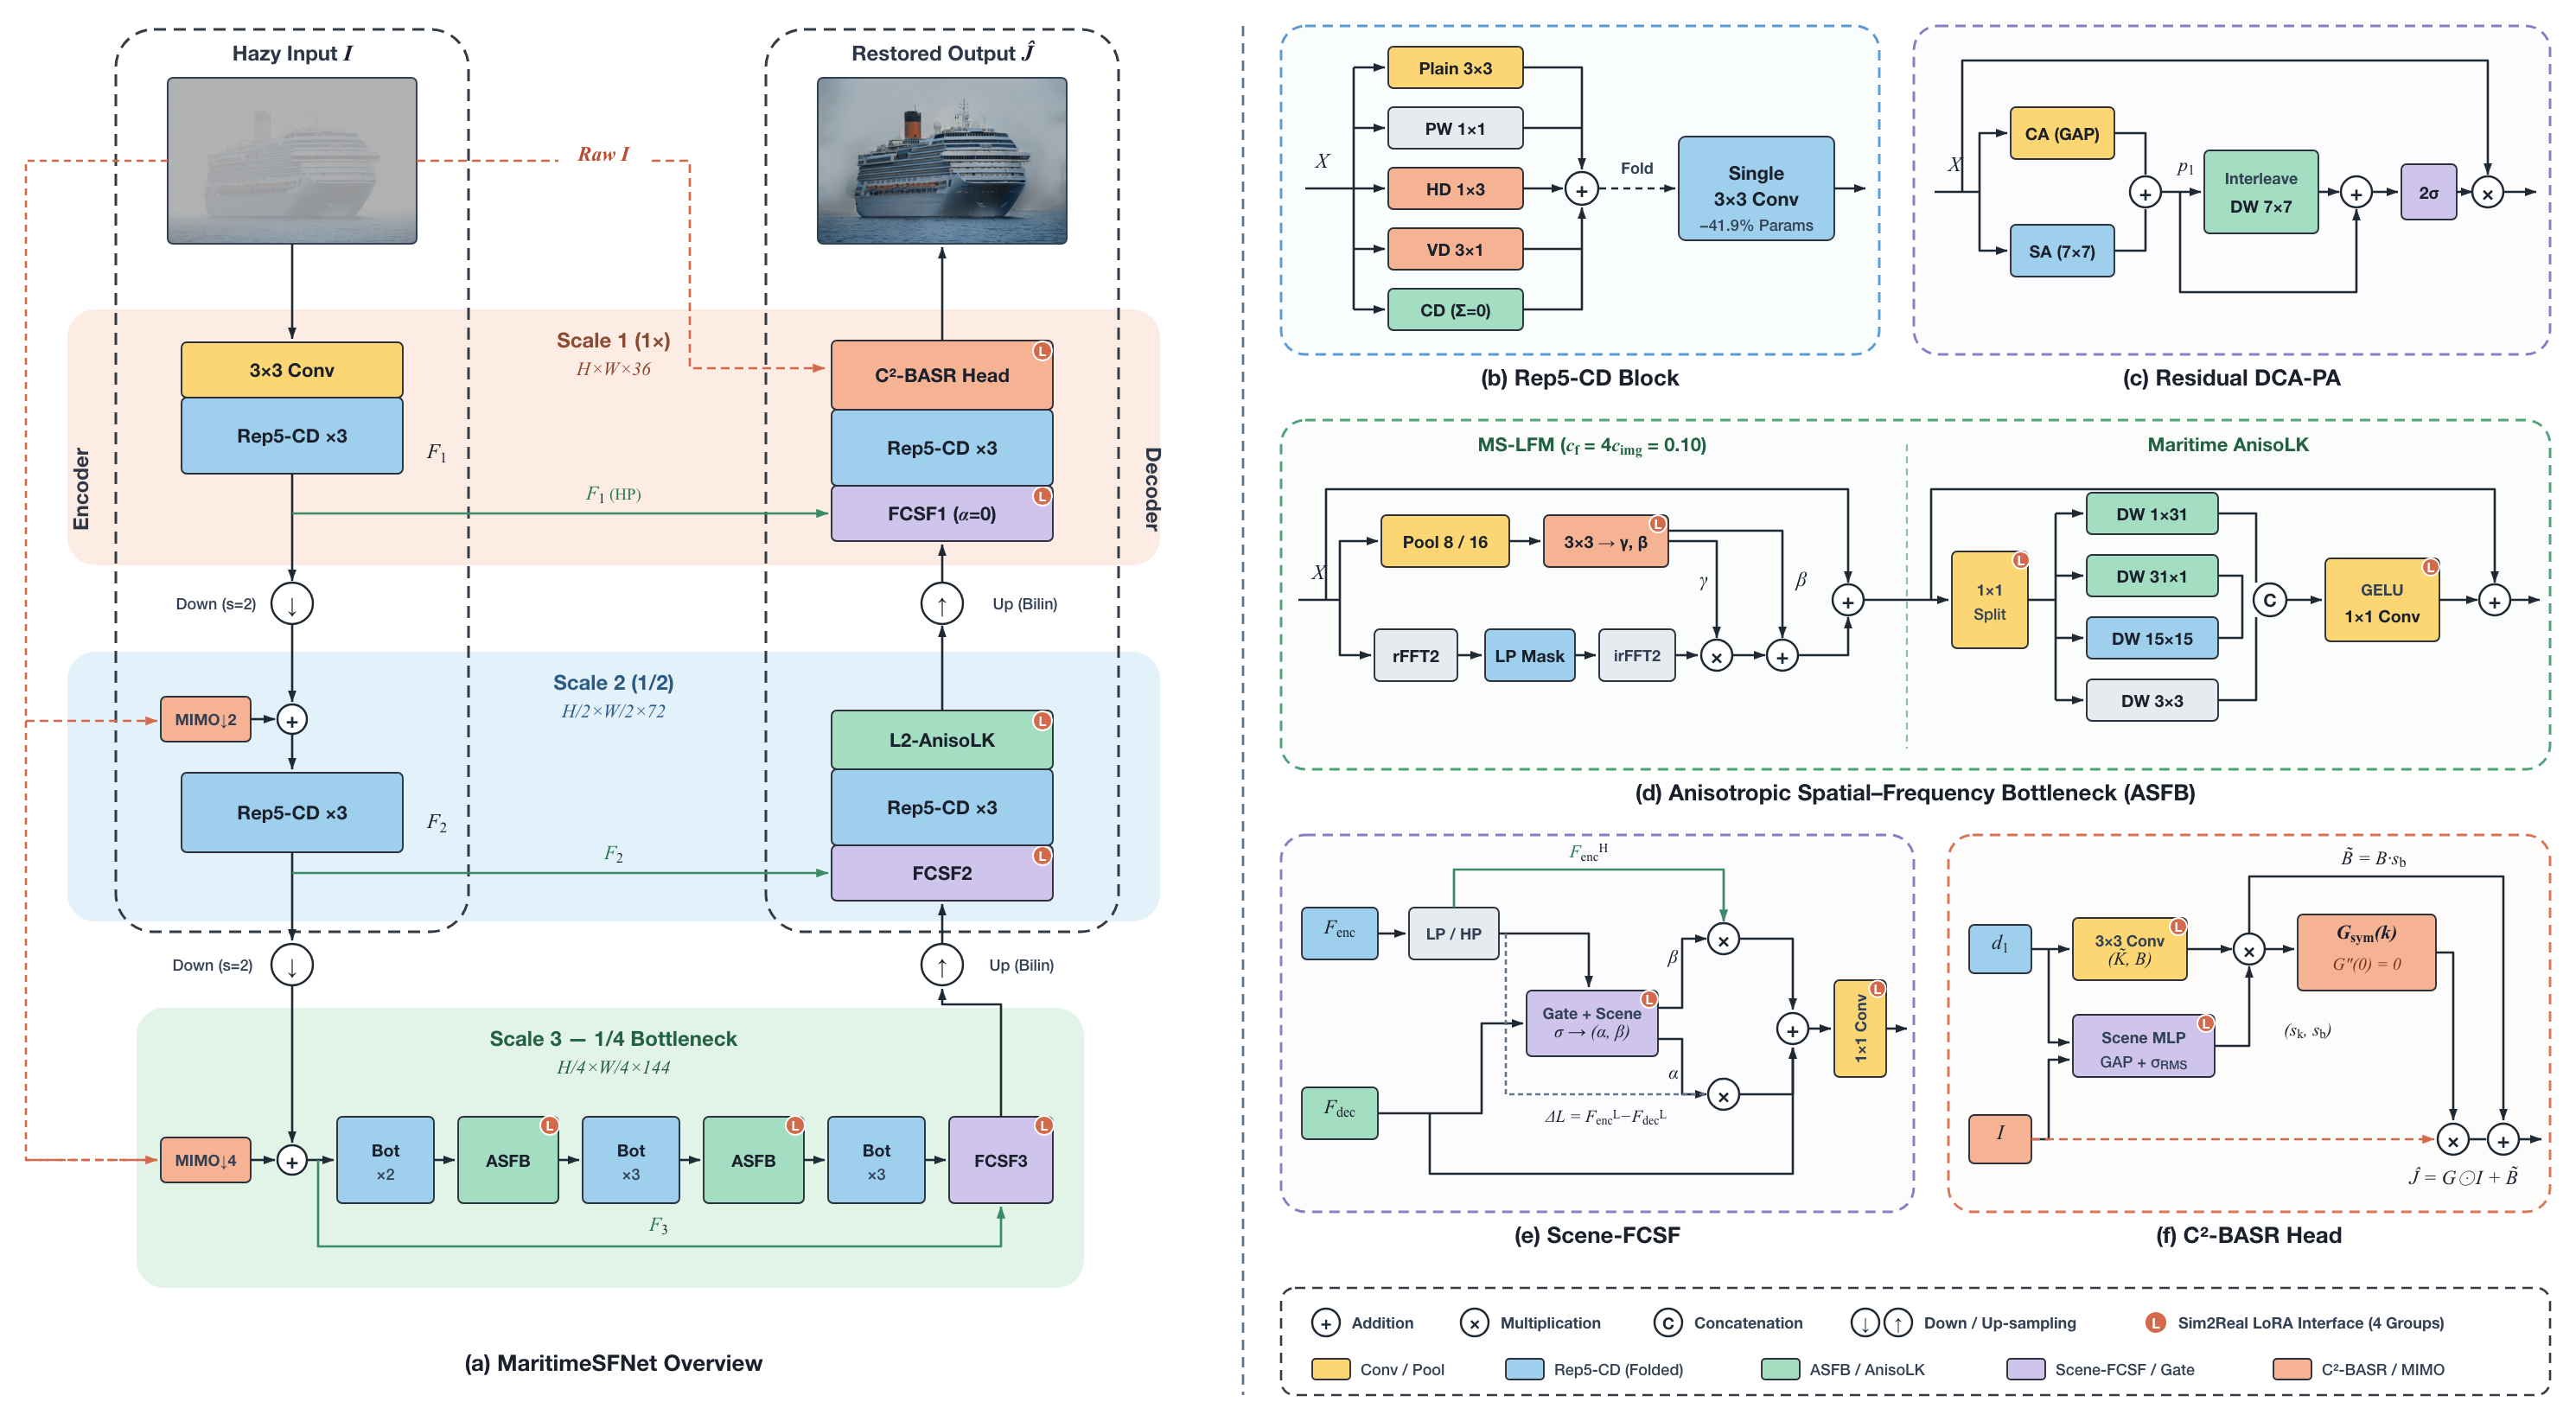
\includegraphics[width=\textwidth]{arch_v4.png}
\caption{Complete architecture of \textbf{MaritimeSFNet} (\texttt{014d}). \textbf{(a)}~Overall three-scale, normalization-free encoder--decoder ($s_{\max}=4$, widths $36/72/144$) with zero-initialized multi-scale input injection (\texttt{MIMO}), bilinear anti-grid upsampling, strict high-pass full-resolution skip ($\alpha_1\equiv 0$), and raw hazy radiance skip $I$ into the physics reconstruction head. Circled \texttt{L} badges denote the four domain-sensitive parameter groups exposed for downstream real-sea-fog LoRA adaptation while the folded local backbone remains frozen. \textbf{(b)}~Five-branch spectral-prior reparameterizable block (\texttt{Rep5-CD}) with zero-DC center-difference branch ($\Sigma=0$) and lossless folding into a single $3\times 3$ convolution ($-41.9\%$ parameters). \textbf{(c)}~Deadlock-free residual \texttt{DCA-PA} bottleneck attention. \textbf{(d)}~Anisotropic Spatial--Frequency Bottleneck (\texttt{ASFB}) coupling physics-aligned \texttt{MS-LFM} ($c_f=4c_{\mathrm{img}}=0.10$) and four-group translation-equivariant \texttt{AnisoLK}. \textbf{(e)}~Scene-aware convex skip fusion (\texttt{Scene-FCSF}). \textbf{(f)}~$C^2$ zero-curvature \texttt{BASR} head ($G''(0)=0$) with global RMS-contrast scene gating.}
\label{fig:arch}
\end{figure*}

To ground architectural decisions in real maritime statistics rather than assumptions, we first perform a train-free physical analysis of the haze residual field $V(x)=I(x)-J(x)$ across all 283 scenes of the Open-Water Haze (OWH) internal validation benchmark spanning three visibility tiers: Dense ($n=94$), Moderate ($n=95$), and Mist ($n=94$). Three empirical laws emerge consistently across all subsets (Fig.~\ref{fig:spectral}(a)):
\begin{itemize}
    \item \textbf{Dominant Low-Band Veil:} Radial 2D Fourier power decomposition reveals that \textbf{86.3\%} (Dense), \textbf{87.0\%} (Moderate), and \textbf{87.3\%} (Mist) of total residual power concentrates below normalized spatial frequency $r_{\mathrm{img}} = 0.02$ Nyquist. Meanwhile, \textbf{8.4\%--9.2\%} lies in the $0.02\text{--}0.15$ mid-band carrying distant ship superstructures, masts, cranes, and horizon boundaries, with only $4.0\%\text{--}4.4\%$ above $0.15$.
    \item \textbf{Directional Depth Anisotropy:} Comparing mean normalized vertical versus horizontal residual gradients confirms strong maritime stratification: $|\partial V/\partial y| / |\partial V/\partial x|$ reaches \textbf{1.46$\times$} in Dense (vertical exceeding horizontal in \textbf{89.4\%} of scenes), \textbf{1.36$\times$} in Moderate (\textbf{86.3\%}), and \textbf{1.37$\times$} in Mist (\textbf{88.3\%}).
    \item \textbf{Wide Contrast Dynamic Range:} Global image root-mean-square contrast $\sigma_{\mathrm{RMS}}(I)$ spans a \textbf{2.11$\times$} operating range from Dense ($0.0658 \pm 0.0292$) through Moderate ($0.0964 \pm 0.0322$) to Mist ($0.1391 \pm 0.0346$), confirming that a single fixed aggressiveness setting cannot serve both regimes without under-dehazing dense fog or overshooting light mist.
\end{itemize}

% -----------------------------------------------------------------------------
\subsection{Overall Three-Scale Backbone and Scale--Bandwidth Alignment}
\label{sec:backbone}

A recurring design error in multi-scale image restoration is borrowing four-scale ($s=8$) or five-scale ($s=16$) U-Net hierarchies from semantic segmentation and applying fixed-cutoff Fourier filters at the deepest bottleneck. The following proposition shows why over-deep downsampling mathematically degrades sea-fog veil modeling.

\begin{proposition}[Scale--Bandwidth Alignment]
\label{prop:scale}
Let an input image of spatial size $H\times W$ have Nyquist radial frequency $N_1 = \min(H,W)/2$. After $L$ stride-2 downsampling stages (total stride $s=2^L$), the bottleneck feature grid has Nyquist frequency $N_s = N_1/s$. A radial low-pass filter applied in the bottleneck feature domain with normalized cutoff $c_f \in (0,1]$ corresponds in the original image normalized frequency coordinate $r_{\mathrm{img}} = \sqrt{\omega_x^2 + \omega_y^2}/N_1$ to an effective physical cutoff frequency and 2D spectral coverage area:
\begin{equation}
c_{\mathrm{img}} = \frac{c_f}{s}, \qquad \Omega_{\mathrm{2D}}(s) = \pi\,c_{\mathrm{img}}^2 = \frac{\pi\,c_f^2}{s^2}.
\label{eq:scale_bw}
\end{equation}
\end{proposition}

\begin{proof}
A discrete spatial frequency vector $(\omega_x,\omega_y)$ in image cycles occupies feature-domain normalized radius $r_f = \sqrt{\omega_x^2+\omega_y^2}/N_s = s\sqrt{\omega_x^2+\omega_y^2}/N_1 = s\,r_{\mathrm{img}}$. Thus, the feature-domain passband $r_f \le c_f$ maps identically to $r_{\mathrm{img}} \le c_f/s$. Integrating over the circular passband disk in the 2D normalized frequency plane gives $\Omega_{\mathrm{2D}}(s) = \pi(c_f/s)^2 = \pi c_f^2 / s^2$.
\end{proof}

Proposition~\ref{prop:scale} yields an immediate architectural consequence (illustrated in Fig.~\ref{fig:motivation}(b) and overlaid on real OWH spectra in Fig.~\ref{fig:spectral}(a)). For a standard feature-domain cutoff $c_f = 0.08\text{--}0.10$:
\begin{itemize}
    \item At \textbf{$s=4$ (3-scale, 1/4 bottleneck)}, $c_{\mathrm{img}} = 0.020\text{--}0.025$ Nyquist ($5.1\text{--}6.4$ cycles per $512$\,px), matching the measured $86\%\text{--}87\%$ maritime haze veil band with $100\%$ reference 2D area.
    \item At \textbf{$s=8$ (4-scale, 1/8 bottleneck)}, $c_{\mathrm{img}}$ halves to $0.010$ and 2D spectral area collapses to \textbf{25\%}, missing spatial fog banks across $0.01\text{--}0.025$ Nyquist.
    \item At \textbf{$s=16$ (5-scale, 1/16 bottleneck)}, $c_{\mathrm{img}}$ collapses to $0.005$ (\textbf{6.25\%} area), degenerating the bottleneck filter into a near-DC scalar bias.
\end{itemize}

Accordingly, MaritimeSFNet adopts a \textbf{three-scale normalization-free hierarchy} ($s\in\{1, 2, 4\}$) with channel widths $(C_1, C_2, C_3) = (36, 72, 144)$ and block depths $(3, 3, 8)$ (Fig.~\ref{fig:arch}(a)). Three deliberate backbone choices support physical fidelity:
\begin{enumerate}
    \item \textbf{Strict Normalization-Free Backbone:} LayerNorm and InstanceNorm subtract per-channel spatial means and divide by channel variance, directly discarding the absolute DC brightness and airlight chromaticity cues required by~\eqref{eq:koschmieder}. Removing normalization layers across all stages preserves radiometric consistency while stabilizing training via zero-initialized residual gates.
    \item \textbf{Zero-Initialized Multi-Scale Input (\texttt{MIMO}) Without Competing Deep Supervision:} Bilinearly downsampled hazy images $I_{1/2}$ and $I_{1/4}$ are projected via zero-initialized $3\times 3$ convolutions into the entrances of Scale~2 and Scale~3, supplying alias-free raw atmospheric veil cues directly to the bottleneck. Crucially, unlike generic multi-output U-Nets, we deliberately omit intermediate $1/2$ and $1/4$ pixel-space auxiliary losses: our controlled ablation (\texttt{014c} vs.\ \texttt{014b}, Section~\ref{sec:ablation}) proves that forcing low-resolution bottleneck features to regress RGB directly competes with decoder representation learning in dense and moderate sea fog.
    \item \textbf{Anti-Grid Bilinear Upsampling:} Strided $3\times 3$ convolutions perform encoder downsampling, while decoder upsampling replaces sub-pixel shuffling (\texttt{PixelShuffle}) with $2\times$ bilinear interpolation followed by $3\times 3$ convolution, preventing $2\times 2$ periodic checkerboard transitions across smooth ocean surfaces and hazy skies.
\end{enumerate}

% -----------------------------------------------------------------------------
\subsection{Spectral-Prior Reparameterization (\texorpdfstring{\texttt{Rep5-CD}}{Rep5-CD}) and Residual \texorpdfstring{\texttt{DCA-PA}}{DCA-PA}}
\label{sec:rep5}

While the bottleneck removes the $0\text{--}0.025$ veil, maritime navigation safety critically depends on recovering crisp $0.02\text{--}0.15$ mid-band vessel contours, bridge superstructures, masts, and harbor cranes without corrupting the DC airlight baseline. Each local residual block in MaritimeSFNet (\texttt{Enc1/2}, \texttt{Bot1--3}, \texttt{Dec1/2}) employs a five-branch anisotropic reparameterizable operator \textbf{AnisoRepConv $3\times 3$ (\texttt{Rep5-CD})} (Fig.~\ref{fig:arch}(b)):
\begin{equation}
\mathcal{F}_{\mathrm{rep}}(X) = \Big(W_{\mathrm{plain}} + W_{\mathrm{pw}} + W_{\mathrm{hd}}^{\mathrm{eff}} + W_{\mathrm{vd}}^{\mathrm{eff}} + W_{\mathrm{cd}}^{\mathrm{eff}}\Big) * X + b_{\mathrm{eq}},
\label{eq:rep5}
\end{equation}
combining a standard $3\times 3$ plain branch $W_{\mathrm{plain}}$, a $1\times 1$ zero-padded pointwise branch $W_{\mathrm{pw}}$, horizontal and vertical first-order difference branches $W_{\mathrm{hd}}^{\mathrm{eff}}, W_{\mathrm{vd}}^{\mathrm{eff}}$ (targeting horizontal sea--sky horizons and vertical ship masts/piles), and an isotropic \textbf{Center Difference (\texttt{CD})} branch parameterized from unconstrained weights $W_{\mathrm{cd}}\in\mathbb{R}^{C\times C\times 3\times 3}$ via:
\begin{equation}
W_{\mathrm{cd}}^{\mathrm{eff}}[u,v] = W_{\mathrm{cd}}[u,v] - \left(\sum_{p=-1}^{1}\sum_{q=-1}^{1} W_{\mathrm{cd}}[p,q]\right)\delta(u,v),
\label{eq:cd_kernel}
\end{equation}
where $\delta(u,v)$ equals $1$ at the kernel center $(0,0)$ and $0$ elsewhere.

\begin{proposition}[Zero-DC Spectral Isolation and Exact Linear Folding]
\label{prop:cd}
For any unconstrained weight tensor $W_{\mathrm{cd}}$, the effective center-difference kernel~\eqref{eq:cd_kernel} satisfies exact zero-DC response $\widehat{W}_{\mathrm{cd}}^{\mathrm{eff}}(0,0) \equiv 0$, acting strictly as a zero-mean isotropic bandpass/high-pass operator (similarly $\widehat{W}_{\mathrm{hd}}^{\mathrm{eff}}(0,0) = \widehat{W}_{\mathrm{vd}}^{\mathrm{eff}}(0,0) \equiv 0$). Furthermore, because convolution is linear in its kernel, all five training branches fold algebraically into a single dense $3\times 3$ kernel $(W_{\mathrm{eq}}, b_{\mathrm{eq}})$ with zero numerical approximation error and zero additional inference FLOPs.
\end{proposition}

\begin{proof}
Summing~\eqref{eq:cd_kernel} over its $3\times 3$ spatial support yields $\widehat{W}_{\mathrm{cd}}^{\mathrm{eff}}(0,0) = \sum_{u,v} W_{\mathrm{cd}}^{\mathrm{eff}}[u,v] = \sum_{u,v} W_{\mathrm{cd}}[u,v] - \sum_{p,q} W_{\mathrm{cd}}[p,q] \equiv 0$. The same identity holds for $W_{\mathrm{hd}}^{\mathrm{eff}} = [w, 0, -w]$ and $W_{\mathrm{vd}}^{\mathrm{eff}} = [w, 0, -w]^{\top}$. By distributivity of 2D convolution over kernel addition, $\sum_k (W_k^{\mathrm{eff}} * X) = (\sum_k W_k^{\mathrm{eff}}) * X$, guaranteeing bit-exact equivalence after merging.
\end{proof}

\begin{figure*}[t]
\centering
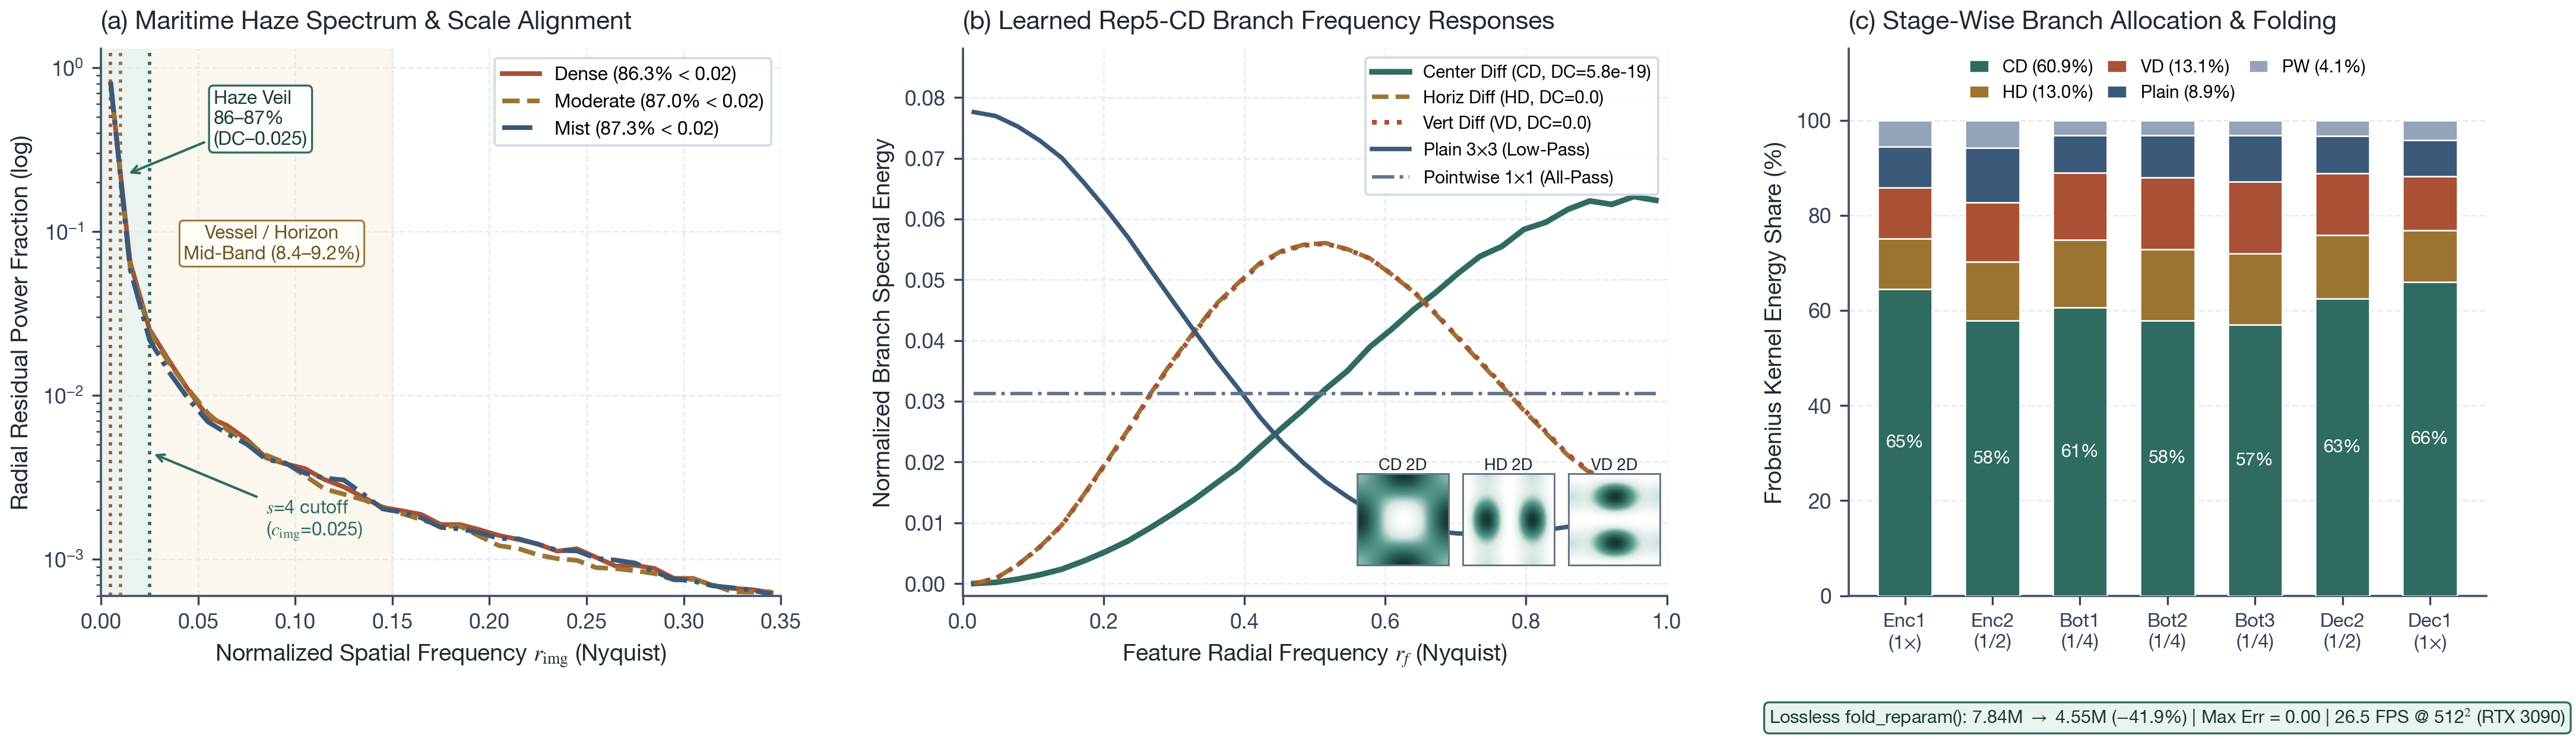
\includegraphics[width=\textwidth]{fig2_spectral_cd_folding.png}
\caption{Empirical spectral physics of maritime sea fog and learned spectral specialization of \texttt{Rep5-CD}. \textbf{(a)}~Radial power fraction of the haze residual $I-J$ across 283 OWH images: $86.3\%\text{--}87.3\%$ resides below $0.02$ Nyquist (matching our $s=4$ cutoff $c_{\mathrm{img}}=0.025$), whereas $s=8$ and $s=16$ cutoffs collapse deeply inside the veil band. \textbf{(b)}~Learned radial FFT responses of the five \texttt{Rep5-CD} branches in trained \texttt{014d} with 2D spectrum insets: \texttt{CD} achieves exact zero DC ($5.75\times 10^{-19}$) with an isotropic high/mid-band ring, \texttt{HD}/\texttt{VD} peak cleanly at mid frequencies, and \texttt{Plain} captures low frequencies. \textbf{(c)}~Stage-wise Frobenius energy share across \texttt{Enc1}--\texttt{Dec1}: \texttt{CD} carries $57\%\text{--}66\%$ ($60.9\%$ overall) and \texttt{HD+VD} carries $26.1\%$ (peaking at $30.0\%$ in the $1/4$ bottleneck), while \texttt{fold\_reparam()} compresses $7.84\text{M}\to 4.55\text{M}$ parameters ($-41.9\%$) with exact $0.00$ error.}
\label{fig:spectral}
\end{figure*}

Unlike plain convolutions that must implicitly trade off DC bias against edge gradients during optimization, \texttt{Rep5-CD} structurally decouples the gradient landscape during training: \texttt{CD}, \texttt{HD}, and \texttt{VD} cannot leak DC haze shifts, forcing them to specialize exclusively in vessel edges and mid-band structure, while \texttt{Plain} and \texttt{PW} manage smooth radiometric continuity. As measured directly on trained \texttt{014d} weights (Fig.~\ref{fig:spectral}(b)--(c)), the network autonomously allocates \textbf{60.9\%} of Frobenius kernel energy to \texttt{CD} (measured DC ratio $5.75\times 10^{-19}$) and \textbf{26.1\%} to \texttt{HD+VD} (peaking at $30.0\%$ in the $1/4$ bottleneck).

\textbf{Deadlock-Free Residual Bottleneck Attention (\texttt{DCA-PA}):} Inside the eight $1/4$-scale bottleneck blocks (\texttt{Bot1--3}), each \texttt{Rep5-CD} residual block is followed by a lightweight normalization-free Dual-Domain Channel--Pixel Attention module (\texttt{DCA-PA}, Fig.~\ref{fig:arch}(c)). Given feature map $x\in\mathbb{R}^{C\times H_4\times W_4}$, we compute a broadcastable global channel prior $w_{\mathrm{ca}} = \mathrm{MLP}_{\mathrm{ca}}(\mathrm{GAP}(x))\in\mathbb{R}^{C\times 1\times 1}$ and a spatial prior $w_{\mathrm{sa}} = \mathrm{Conv}_{7\times 7}([\mathrm{Mean}_c(x), \mathrm{Max}_c(x)])\in\mathbb{R}^{1\times H_4\times W_4}$, summing them into $p_1 = w_{\mathrm{ca}} + w_{\mathrm{sa}}\in\mathbb{R}^{C\times H_4\times W_4}$. Rather than stopping at channel-shared spatial weighting, we interleave $x$ and $p_1$ channel-by-channel and pass them through a zero-initialized grouped $7\times 7$ depthwise convolution $\mathrm{PA}_0$ in a \emph{residual} refinement form:
\begin{equation}
p_2 = p_1 + \mathrm{PA}_0\big(\mathrm{Interleave}(x, p_1)\big), \qquad y = x \odot \big(2\,\sigma(p_2)\big).
\label{eq:dcapa}
\end{equation}
Two properties make~\eqref{eq:dcapa} strictly superior to direct sequential pixel-attention gating: (i)~at initialization, zero-initialized projections give $p_2\equiv 0 \Rightarrow 2\sigma(p_2)\equiv 1$, preserving strict identity mapping and DC statistics; (ii)~the residual bypass $p_1$ avoids the zero-gradient deadlock that arises when a zero-initialized $\mathrm{PA}_0$ sits serially after $p_1$, allowing both global channel color balance and per-channel $7\times 7$ spatial separation of bright vessels from hazy skies to train smoothly from iteration~1.

% -----------------------------------------------------------------------------
\subsection{Anisotropic Spatial--Frequency Bottleneck (\texorpdfstring{\texttt{ASFB}}{ASFB}) and Mid-Band \texorpdfstring{\texttt{L2-AnisoLK}}{L2-AnisoLK}}
\label{sec:asfb}

At the $1/4$-scale bottleneck ($128\times 128$ for a $512^2$ input), MaritimeSFNet interleaves two \textbf{Anisotropic Spatial--Frequency Bottleneck (\texttt{ASFB})} modules after \texttt{Bot1} and \texttt{Bot2} (Fig.~\ref{fig:arch}(a,d)). Each \texttt{ASFB} couples two complementary, strictly zero-initialized pathways designed specifically for open-water horizon geometry:

\textbf{1) Multi-Scale Low-Frequency Modulation (\texttt{MS-LFM}):} Applying Proposition~\ref{prop:scale} with target maritime veil band $c_{\mathrm{img}} = 0.025$ gives exact feature-domain cutoff $c_f = 4\,c_{\mathrm{img}} = 0.10$. For bottleneck tensor $X\in\mathbb{R}^{C_3\times H_4\times W_4}$, we apply an orthonormal real 2D Fourier transform $\mathcal{F}(\cdot)$, multiply by a smooth radial sigmoid low-pass mask $M_{\mathrm{lp}}(r_f; c_f)$, and invert to obtain the clean low-frequency component $X_{\mathrm{low}} = \mathcal{F}^{-1}(M_{\mathrm{lp}} \odot \mathcal{F}(X))$. To adapt modulation spatially across both global ocean illumination and localized coastal fog banks, we extract dual adaptive average pooling grids at $8\times 8$ and $16\times 16$, upsample and concatenate them, and predict spatial scale and shift fields $(\gamma, \beta)$ via a zero-initialized $3\times 3$ modulation head:
\begin{equation}
\begin{aligned}
X_{\mathrm{freq}} = X &+ \gamma(X_{\mathrm{pool},8}, X_{\mathrm{pool},16}) \odot X_{\mathrm{low}} \\
                      &+ \beta(X_{\mathrm{pool},8}, X_{\mathrm{pool},16}).
\end{aligned}
\label{eq:mslfm}
\end{equation}
Because \texttt{MS-LFM} contains zero normalization layers and is initialized identically to zero ($\gamma,\beta \equiv 0$), it preserves DC color calibration while directly attenuating the $86\%\text{--}87\%$ sea-fog veil.

\textbf{2) Translation-Equivariant Maritime Anisotropic Large-Kernel Context (\texttt{AnisoLK}):} To model the $1.36\text{--}1.46\times$ vertical-over-horizontal depth anisotropy without the non-local sky-to-hull halo contamination observed in dot-product attention, the second branch splits a $1\times 1$-projected bottleneck tensor into four equal channel groups ($C_3/4 = 36$ channels each) and applies parallel depthwise convolutions:
\begin{equation}
\begin{aligned}
\mathcal{G}(U) = \mathrm{Concat}\Big(&\mathrm{DW}_{1\times 31}(U_1),\; \mathrm{DW}_{31\times 1}(U_2), \\
&\mathrm{DW}_{15\times 15}(U_3),\; \mathrm{DW}_{3\times 3}(U_4)\Big),
\end{aligned}
\label{eq:anisolK}
\end{equation}
followed by GELU activation and a zero-initialized $1\times 1$ residual projection:
\begin{equation}
X_{\mathrm{out}} = X_{\mathrm{freq}} + \mathrm{Conv}_{1\times 1,0}\big(\mathrm{GELU}(\mathcal{G}(\mathrm{Conv}_{1\times 1}(X_{\mathrm{freq}})))\big).
\label{eq:aniso_res}
\end{equation}
Each kernel plays a dedicated physical role at $1/4$ scale: $\mathrm{DW}_{1\times 31}$ spans \textbf{124\,px} horizontally along iso-depth sea--sky strips to distinguish localized white ship cabins from continuous fog bands; $\mathrm{DW}_{31\times 1}$ spans \textbf{124\,px} vertically to track smooth exponential transmission decay $t(y)=\exp(-\beta d(y))$ from sky to near-field water; $\mathrm{DW}_{15\times 15}$ ($60$\,px span) captures patchy advection fog pockets; and $\mathrm{DW}_{3\times 3}$ anchors crisp foreground vessel edges. Because every branch is strictly convolutional, translation equivariance and spatial locality are guaranteed by construction.

\begin{figure*}[t]
\centering
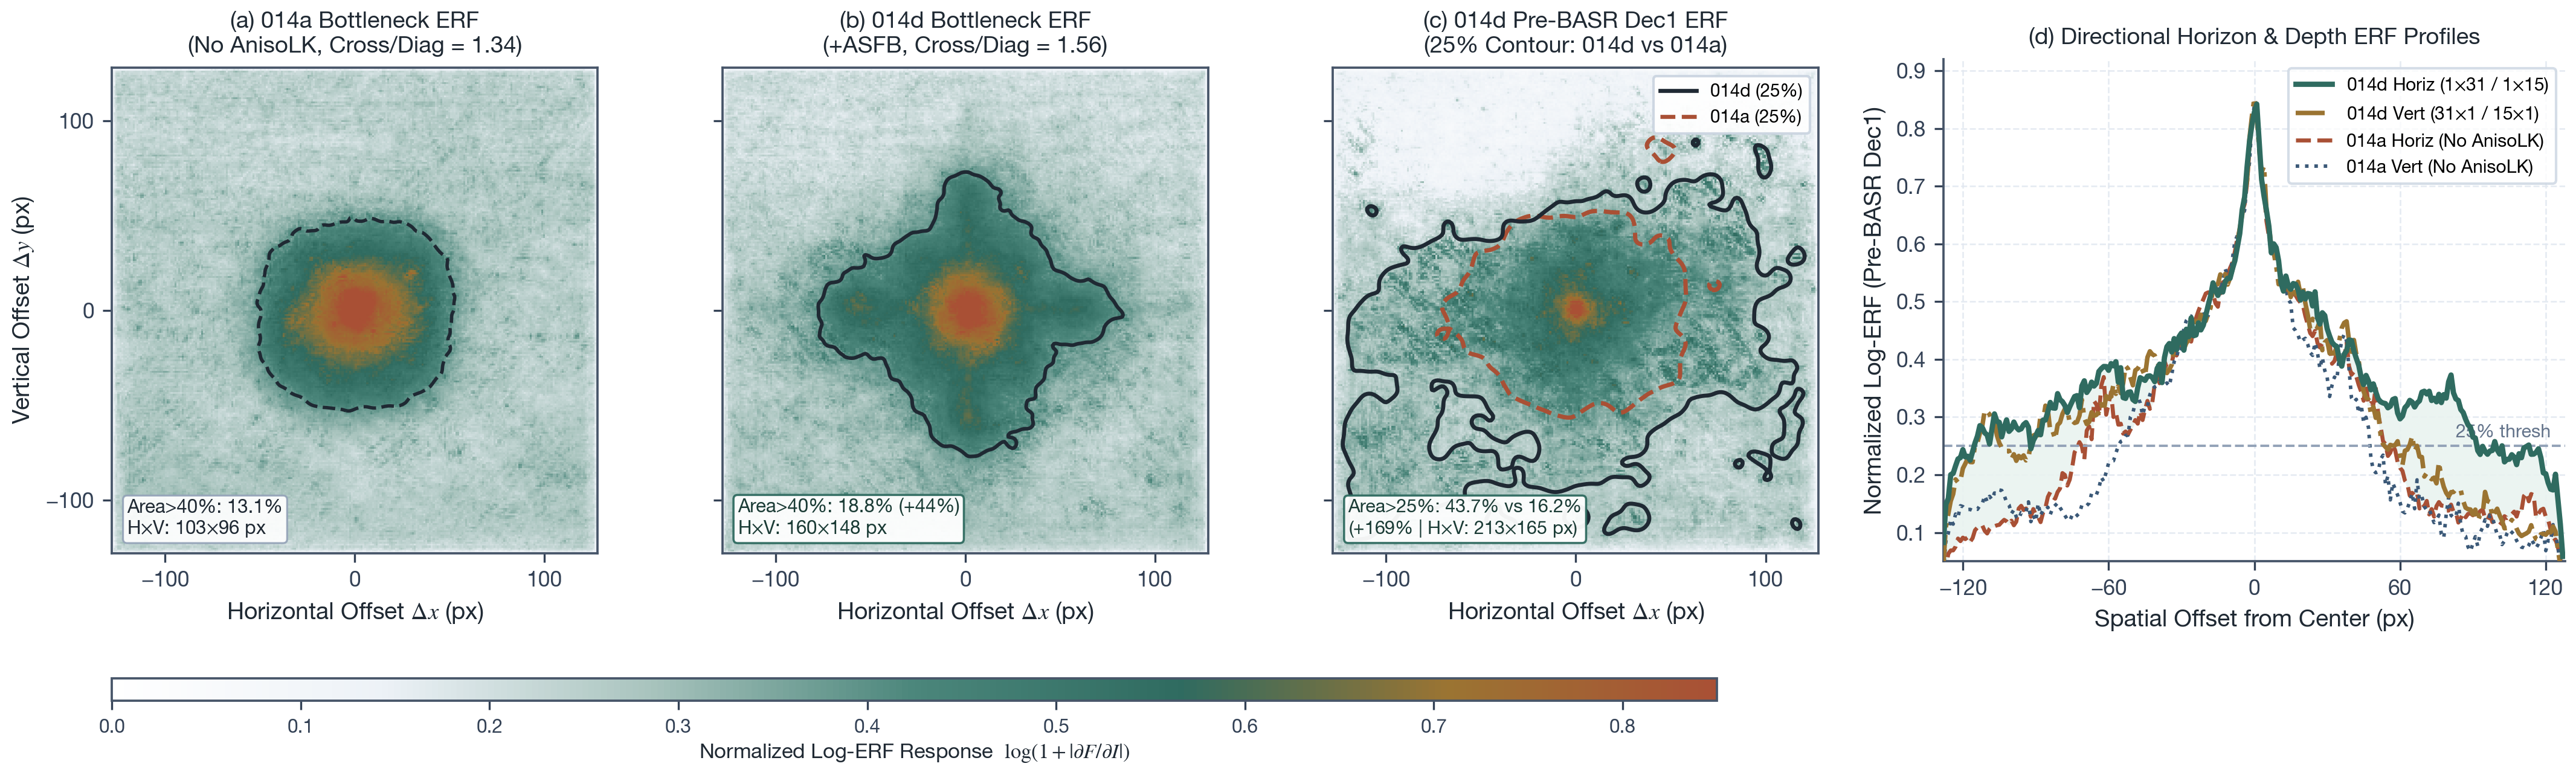
\includegraphics[width=\textwidth]{fig3_erf_anisotropy.png}
\caption{Train-free Effective Receptive Field (ERF) analysis averaged over 30 real OWH maritime images ($256\times 256$ crops), measured at pre-BASR feature tensors to avoid domination by the direct pixel skip $I$. \textbf{(a)}~Without \texttt{AnisoLK} (\texttt{014a}), the bottleneck ERF forms a compact square ($\text{Area}{>}40\% = 13.1\%$, $103\times 96$\,px, cross/diag $=1.34$). \textbf{(b)}~With \texttt{ASFB} (\texttt{014d}), the bottleneck ERF forms a pronounced horizontal/vertical maritime cross ($\text{Area}{>}40\% = 18.8\%$, $+44\%$, $160\times 148$\,px, cross/diag $=1.56$). \textbf{(c)}~At the pre-BASR decoder (\texttt{Dec1}), Gaussian-smoothed $25\%$ contours reveal a $+169\%$ ERF area expansion ($43.7\%$ vs.\ $16.2\%$, $213\times 165$\,px) driven jointly by \texttt{ASFB} and \texttt{L2-AnisoLK}. \textbf{(d)}~1D horizontal and vertical log-ERF profiles through the center confirming sustained long-range horizon and depth sensitivity.}
\label{fig:erf}
\end{figure*}

\textbf{Mid-Band 1/2-Scale Refinement (\texttt{L2-AnisoLK}):} To bridge the gap between the $1/4$-scale bottleneck ($60\text{--}124$\,px spans) and full-resolution local convolutions, we append a lightweight half-scale \texttt{L2-AnisoLK} block ($\mathrm{DW}_{1\times 15}$, $\mathrm{DW}_{15\times 1}$, $\mathrm{DW}_{7\times 7}$, $\mathrm{DW}_{3\times 3}$; physical spans $14\text{--}30$\,px) directly after \texttt{Dec2} at a cost of only $+0.018\text{M}$ parameters. This targets the exact $0.02\text{--}0.15$ mid-band wavelength of mid-range ship superstructures, bridge windows, and rigging. Train-free ERF diagnostics (Fig.~\ref{fig:erf}) confirm that \texttt{ASFB} and \texttt{L2-AnisoLK} expand the pre-BASR \texttt{Dec1} effective receptive field area above $25\%$ response by \textbf{+169.3\%} ($0.437$ vs.\ $0.162$, $213\times 165$\,px vs.\ $127\times 100$\,px) while increasing bottleneck cross-to-diagonal anisotropy from $1.343$ to $1.557$.

% -----------------------------------------------------------------------------
\subsection{Scene-Aware Frequency-Decoupled Convex Skip Fusion (\texorpdfstring{\texttt{Scene-FCSF}}{Scene-FCSF})}
\label{sec:fcsf}

Standard U-Net skip connections concatenate or add raw shallow encoder features $F_{\mathrm{enc}}$ directly onto dehazed decoder features $F_{\mathrm{dec}}$. Because shallow features retain strong unprocessed sea-fog airlight in their low-frequency band, unconstrained skip connections re-inject haze back into the decoder; conversely, eliminating skip connections loses crisp ship-edge localization.

We resolve this tension by decomposing both encoder and decoder features at scale $l\in\{1,2,3\}$ via a smooth, alias-free low-pass operator $\mathcal{L}(\cdot)$ (stride-2 average pooling followed by bilinear upsampling):
\begin{equation}
F^L = \mathcal{L}(F), \qquad F^H = F - F^L.
\label{eq:lp_split}
\end{equation}
We then define \textbf{Scene-Aware Frequency-Decoupled Convex Skip Fusion (\texttt{Scene-FCSF})} (Fig.~\ref{fig:arch}(e)):
\begin{equation}
\begin{aligned}
F_{\mathrm{fuse}} = \mathrm{Conv}_{1\times 1}\!\Big(&\underbrace{(1 - \alpha)\odot F_{\mathrm{dec}}^L + \alpha \odot F_{\mathrm{enc}}^L}_{\text{strictly convex low-band fusion}} \\
&+ F_{\mathrm{dec}}^H + \beta \odot F_{\mathrm{enc}}^H\Big),
\end{aligned}
\label{eq:fcsf}
\end{equation}
which admits the computationally clean residual form $F_{\mathrm{fuse}} = \mathrm{Conv}_{1\times 1}(F_{\mathrm{dec}} + \alpha\odot(F_{\mathrm{enc}}^L - F_{\mathrm{dec}}^L) + \beta\odot F_{\mathrm{enc}}^H)$.

\begin{proposition}[Convex Energy Boundedness and Anti-Leakage]
\label{prop:fcsf}
For any spatial gating map $\alpha(x)\in(0,1)$, the fused low-frequency field $F_{\mathrm{fuse}}^L(x) = (1-\alpha(x))F_{\mathrm{dec}}^L(x) + \alpha(x)F_{\mathrm{enc}}^L(x)$ lies strictly inside the pointwise convex hull of $\{F_{\mathrm{dec}}^L(x), F_{\mathrm{enc}}^L(x)\}$, preventing unbounded gain amplification. Setting $\alpha_1\equiv 0$ at full resolution ($1\times$) completely eliminates raw low-frequency haze passthrough while preserving high-pass edge injection $\beta_1 \odot F_{\mathrm{enc}}^H$.
\end{proposition}

Crucially, local $6\text{--}12$\,px receptive fields cannot reliably distinguish whether a locally flat bright patch belongs to dense sea fog (requiring $\alpha\to 0$ to block haze) or clear bright mist/sky (benefiting from higher $\alpha$ to preserve natural tone). Therefore, \texttt{Scene-FCSF} sums a lightweight local depthwise gate with a zero-initialized \textbf{global Scene Context Gate} driven by global average pooling of $(F_{\mathrm{dec}}, F_{\mathrm{enc}}^L - F_{\mathrm{dec}}^L, |F_{\mathrm{enc}}^H|)$:
\begin{equation}
\alpha = \sigma\big(z_{\alpha}^{\mathrm{loc}} + z_{\alpha}^{\mathrm{glob}} + b_{\alpha}\big), \qquad \beta = \sigma\big(z_{\beta}^{\mathrm{loc}} + z_{\beta}^{\mathrm{glob}}\big),
\label{eq:fcsf_gate}
\end{equation}
with deep-dominant initialization $b_{\alpha}=-1.2$ ($\alpha_0\approx 0.231$, giving the dehazed decoder $77\%$ initial control). At full $1\times$ resolution (\texttt{FCSF1}), $\alpha_1$ is structurally fixed to $0$ so only detail gate $\beta_1$ operates. As verified across 283 OWH scenes (Fig.~\ref{fig:basr}(b)), \texttt{Scene-FCSF} autonomously learns monotonic visibility adaptation without any haze-density labels: mean $\alpha_3$ rises smoothly from \textbf{0.316} (Dense) $\to$ \textbf{0.352} (Moderate) $\to$ \textbf{0.460} (Mist), $\alpha_2$ rises \textbf{0.431 $\to$ 0.468 $\to$ 0.534}, while detail injection $\beta_1$ intensifies under heavier fog (\textbf{0.386} Dense $\to$ \textbf{0.367} Moderate $\to$ \textbf{0.288} Mist).

% -----------------------------------------------------------------------------
\subsection{\texorpdfstring{$C^2$}{C2} Zero-Curvature Bounded Affine Soft Reconstruction (\texorpdfstring{\texttt{$C^2$-BASR}}{C2-BASR})}
\label{sec:basr}

Motivated by the exact atmospheric scattering inverse~\eqref{eq:affine_inv}, the output head maps final decoder features $d_1\in\mathbb{R}^{C_1\times H\times W}$ via a zero-initialized $3\times 3$ convolution into six channels representing multiplicative gain logits $\tilde{K}\in\mathbb{R}^{3\times H\times W}$ and additive airlight bias $B\in\mathbb{R}^{3\times H\times W}$. To avoid both polarity inversion ($G<0$) and $1/t\to\infty$ blow-up in dense fog, an intuitive parameterization bounds $G$ via a shifted sigmoid:
\begin{equation}
G_{\mathrm{sig}}(k) = g_{\min} + (g_{\max} - g_{\min})\,\sigma(k + b_0),
\label{eq:basr_sig}
\end{equation}
with $g_{\min}=0.5$, $g_{\max}=5.0$, and identity bias $b_0 = -\ln 8 \approx -2.0794$ satisfying $G_{\mathrm{sig}}(0)=1$.

However, our paired error attribution of the sigmoid-head prototype (\texttt{014b}, Section~\ref{sec:ablation}) uncovered a systematic $+21\%\text{--}31\%$ excess in \texttt{overshoot\_mse} across all visibility tiers, with mean gain stuck at $1.146\text{--}1.151$ and $5\text{th}$-percentile pixel gain remaining strictly above unity in $95.7\%$ of Mist scenes. The following theorem diagnoses the exact analytical cause and proves our remedy.

\begin{theorem}[Curvature-Induced Overshoot and $C^2$ Zero-Curvature Remedy]
\label{thm:basr}
Let $g_{\min}\in(0,1)$ and $g_{\max}>1$ define the strictly positive gain interval, with $a_- = 1 - g_{\min}$ and $a_+ = g_{\max} - 1$.
\begin{enumerate}
    \item \textbf{Sigmoid Curvature \& Gradient Asymmetry:} For the shifted sigmoid~\eqref{eq:basr_sig} with $g_{\min}=0.5, g_{\max}=5.0$, $\sigma(b_0)=1/9$, yielding first and second derivatives at identity $k=0$:
    \begin{equation}
    G_{\mathrm{sig}}'(0) = \frac{4}{9} \approx 0.444,\quad G_{\mathrm{sig}}''(0) = \frac{28}{81} \approx +0.346 > 0.
    \label{eq:sig_curv}
    \end{equation}
    Consequently, (a)~for any zero-mean local perturbation $k$ with small variance $\sigma_k^2$, Taylor expansion yields positive Jensen gain bias $\mathbb{E}[G_{\mathrm{sig}}(k)] - 1 \approx \frac{14}{81}\sigma_k^2 > 0$; and (b)~sensitivity is severely asymmetric around identity, with $G_{\mathrm{sig}}'(+0.5)/G_{\mathrm{sig}}'(-0.5) = 2.16$, starving negative attenuation updates ($k<0$) relative to positive contrast boosts ($k>0$).
    \item \textbf{$C^2$ Zero-Curvature Piecewise-$\tanh$ Parameterization:} Define the asymmetric piecewise hyperbolic tangent gain (with $g_{\min}=0.5, g_{\max}=4.0 \Rightarrow a_-=0.5, a_+=3.0$):
    \begin{equation}
    G_{\mathrm{sym}}(k) =
    \begin{cases}
    1 + a_+\,\tanh\!\left(\dfrac{k}{a_+}\right), & k \ge 0, \\[8pt]
    1 + a_-\,\tanh\!\left(\dfrac{k}{a_-}\right), & k < 0.
    \end{cases}
    \label{eq:basr_sym}
    \end{equation}
    Then $G_{\mathrm{sym}} \in C^2(\mathbb{R})$ satisfies strict boundedness $G_{\mathrm{sym}}(k)\in(g_{\min}, g_{\max})$, exact identity $G_{\mathrm{sym}}(0)=1$, unit symmetric slope $G_{\mathrm{sym}}'(0^+)=G_{\mathrm{sym}}'(0^-)=1$, and \textbf{exact zero curvature at identity}:
    \begin{equation}
    G_{\mathrm{sym}}''(0^+) = G_{\mathrm{sym}}''(0^-) = 0.
    \label{eq:sym_zero_curv}
    \end{equation}
\end{enumerate}
\end{theorem}

\begin{proof}
For~\eqref{eq:basr_sig}, setting $p=\sigma(b_0)=1/9$ gives $G_{\mathrm{sig}}'(0)=(g_{\max}-g_{\min})p(1-p)=4.5\cdot\frac{1}{9}\cdot\frac{8}{9}=\frac{4}{9}$ and $G_{\mathrm{sig}}''(0)=(g_{\max}-g_{\min})p(1-p)(1-2p)=4.5\cdot\frac{8}{81}\cdot\frac{7}{9}=\frac{28}{81}$. At $k=\pm 0.5$, direct evaluation yields $G_{\mathrm{sig}}'(+0.5)=0.638$ vs.\ $G_{\mathrm{sig}}'(-0.5)=0.295$ (ratio $2.16$).

For~\eqref{eq:basr_sym}, clearly $\tanh(\cdot)\in(-1,1)$ ensures $G_{\mathrm{sym}}(k)\in(1-a_-, 1+a_+)=(g_{\min}, g_{\max})$. Differentiating each branch gives:
\begin{align}
G_{\mathrm{sym}}'(k) &= \operatorname{sech}^2\!\left(\frac{k}{a_\pm}\right), \\
G_{\mathrm{sym}}''(k) &= -\frac{2}{a_\pm}\operatorname{sech}^2\!\left(\frac{k}{a_\pm}\right)\tanh\!\left(\frac{k}{a_\pm}\right).
\end{align}
Taking one-sided limits as $k\to 0^\pm$, $\operatorname{sech}^2(0)=1$ and $\tanh(0)=0$ regardless of $a_+\neq a_-$, establishing $G_{\mathrm{sym}}(0^\pm)=1$, $G_{\mathrm{sym}}'(0^\pm)=1$, and $G_{\mathrm{sym}}''(0^\pm)=0$. Thus $G_{\mathrm{sym}}$ is twice continuously differentiable across $k=0$ with local expansion $G_{\mathrm{sym}}(k) = 1 + k + O(k^3)$ and zero second-order Jensen term $\frac{1}{2}G_{\mathrm{sym}}''(0)\operatorname{Var}(k)\equiv 0$.
\end{proof}

\begin{figure*}[t]
\centering
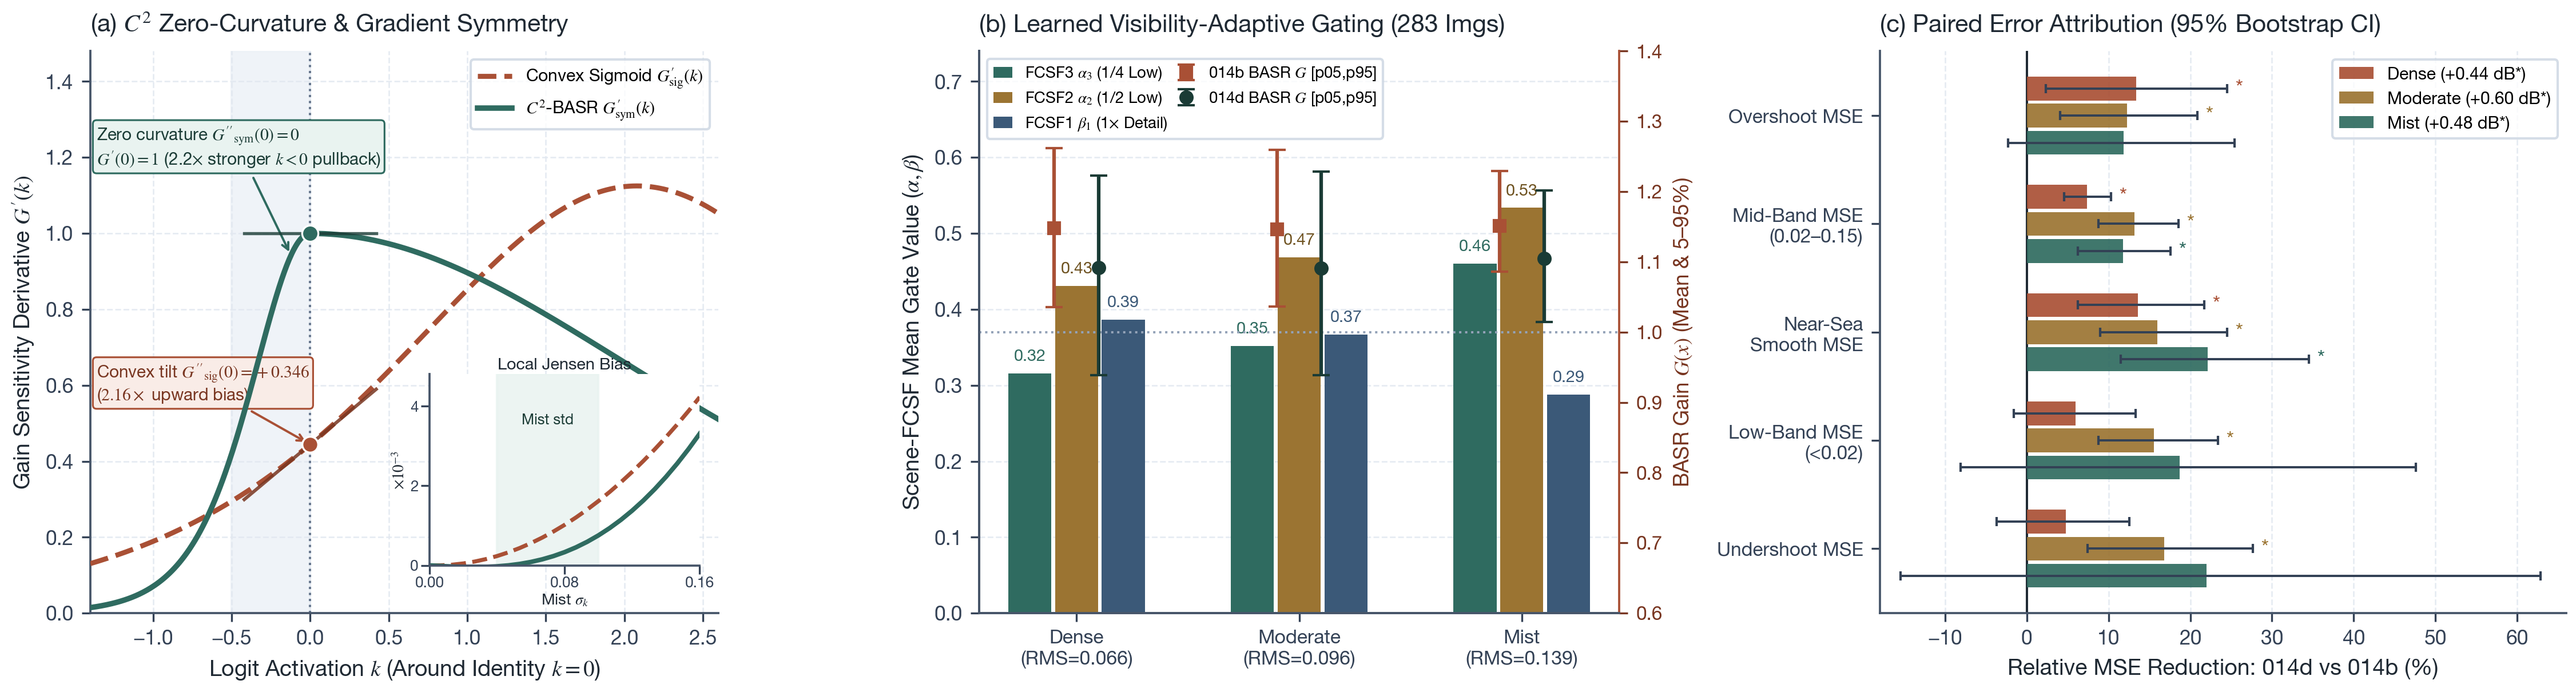
\includegraphics[width=\textwidth]{fig4_basr_curvature_gates.png}
\caption{Analytical proof and empirical verification of \texttt{$C^2$-BASR} and \texttt{Scene-FCSF}. \textbf{(a)}~Gain sensitivity $G'(k)$ around identity $k=0$: \texttt{$C^2$-BASR} achieves a flat zero-curvature peak ($G'(0)=1, G''(0)=0$) with $2.16\times$ stronger negative pullback at $k=-0.25$ ($0.786$ vs.\ $0.364$), cutting local mist-regime Jensen drift by $30\text{--}42\%$ (inset). \textbf{(b)}~Measured gating statistics across all 283 OWH images: \texttt{Scene-FCSF} gates ($\alpha_3, \alpha_2, \beta_1$) shift monotonically with image RMS contrast ($0.066\to 0.139$), while \texttt{$C^2$-BASR} lowers mean gain from $1.15\to 1.09$ and unlocks $<1.0$ attenuation (5th percentile drops below $1.0$ in $70.2\%$ Dense / $76.8\%$ Moderate / $27.7\%$ Mist scenes vs.\ $33.0\% / 30.5\% / 4.3\%$ for \texttt{014b}). \textbf{(c)}~Paired relative MSE reductions of \texttt{014d} vs.\ \texttt{014b} with $95\%$ bootstrap confidence intervals ($^*$ denotes $p<0.05$).}
\label{fig:basr}
\end{figure*}

\textbf{Global RMS-Contrast Scene Gate:} Because maritime visibility spans a $2.11\times$ contrast range, we equip \texttt{$C^2$-BASR} with a lightweight global \textbf{Scene Contrast Gate} (Fig.~\ref{fig:arch}(f)) taking the concatenated scene descriptor $z_{\mathrm{scene}} = [\mathrm{GAP}(d_1),\; \mathrm{GAP}(I),\; \sigma_{\mathrm{RMS}}(I)] \in \mathbb{R}^{C_1+6}$, where $\sigma_{\mathrm{RMS}}(I) = \sqrt{\mathrm{Var}_{u,v}(I) + 10^{-6}}$ is the per-channel spatial contrast standard deviation---a direct physical indicator of sea-fog density. A zero-initialized two-layer MLP outputs global scaling factors $(s_k, s_b) = 2\sigma(\mathrm{MLP}_0(z_{\mathrm{scene}}))\in(0,2)^2$ (strictly $1.0$ at initialization), yielding the final reconstructed clear radiance:
\begin{equation}
\hat{J}(x) = G_{\mathrm{sym}}\!\big(s_k \odot \tilde{K}(x)\big) \odot I(x) + s_b \odot B(x).
\label{eq:basr_final}
\end{equation}
Fig.~\ref{fig:basr}(a)--(b) validates Theorem~\ref{thm:basr} both analytically and empirically: at $k=-0.25$, \texttt{$C^2$-BASR} supplies a $2.16\times$ stronger downward restoring slope ($0.786$ vs.\ $0.364$), increasing the fraction of scenes exhibiting $<1.0$ attenuation ($p_{05}<1.0$) from $4.3\%\to 27.7\%$ in Mist ($6.4\times$), $30.5\%\to 76.8\%$ in Moderate, and $33.0\%\to 70.2\%$ in Dense, while lowering mean gain from $1.151\to 1.105$.

% -----------------------------------------------------------------------------
\subsection{Training Objective and Structural Interface for Sim2Real LoRA}
\label{sec:loss_lora}

To jointly supervise spatial luminance, frequency-band fidelity, and crisp vessel contours without adversarial instability, MaritimeSFNet is trained end-to-end with a composite spatial--spectral--gradient objective:
\begin{equation}
\mathcal{L} = \|\hat{J} - J\|_1 + \lambda_{\mathrm{fft}}\,\|\mathcal{F}(\hat{J}) - \mathcal{F}(J)\|_1 + \lambda_{\mathrm{grad}}\,\|\nabla \hat{J} - \nabla J\|_1,
\label{eq:loss}
\end{equation}
where $\nabla$ denotes discrete Sobel horizontal/vertical gradients ($\lambda_{\mathrm{fft}}=0.05$, $\lambda_{\mathrm{grad}}=0.05$).

Furthermore, real marine sea fog exhibits wavelength-dependent blue-shifted atmospheric light and $3.8\times$ higher inter-channel dispersion than synthetic benchmarks. Rather than fine-tuning all weights under noisy unpaired supervision---which risks corrupting learned ship geometry---MaritimeSFNet natively partitions its parameters into a \textbf{frozen domain-invariant texture backbone} (folded \texttt{Rep5-CD} layers) and \textbf{four physically localized domain-sensitive interfaces} marked by \texttt{L} in Fig.~\ref{fig:arch} and summarized in Table~\ref{tab:lora_groups}.

\begin{table}[t]
\centering
\caption{Native Structural Partition of MaritimeSFNet for Onboard Deployment and Downstream Real-Sea-Fog LoRA Adaptation}
\label{tab:lora_groups}
\renewcommand{\arraystretch}{1.15}
\setlength{\tabcolsep}{3.5pt}
\resizebox{\columnwidth}{!}{%
\begin{tabular}{@{}llll@{}}
\toprule
\textbf{Module Group} & \textbf{Sub-Modules} & \textbf{Post-Pretrain} & \textbf{Physical Domain Role} \\
\midrule
Local Texture & \texttt{Stem, Enc1/2,} & Fold \texttt{Rep5-CD} & Preserves vessel hull, mast, \\
Backbone & \texttt{Dec1/2, Bot} $3{\times}3$ & \& \textbf{Freeze} & \& wave geometry \\
\midrule
Interface~\textcircled{1} & \texttt{ASFB.ms\_lfm.mod} & LoRA ($r{=}8\text{--}16$) & Calibrates blue-shifted $A_c(x)$ \\
Interface~\textcircled{2} & \texttt{AnisoLK} $1{\times}1$ proj & LoRA ($r{=}8$) & Adapts non-uniform depth $t(y)$ \\
Interface~\textcircled{3} & \texttt{Scene-FCSF} gates & LoRA ($r{=}4\text{--}8$) & Re-balances RGB dispersion \\
Interface~\textcircled{4} & \texttt{$C^2$-BASR} + Gate & LoRA ($r{=}4\text{--}8$) & Pixel contrast $G_c$ \& chroma $B_c$ \\
\bottomrule
\end{tabular}}
\end{table}

% =============================================================================
\section{Mechanistic Verification and Causal Ablation}
\label{sec:experiments}
% =============================================================================

\subsection{Controlled Causal Ablation Ladder}
\label{sec:ablation}

To isolate the causal contribution of every design choice without confounding hyperparameter drift, all models are evaluated under an identical controlled 8,000-iteration protocol on the OWH dataset (batch size $16$ at $512\times 512$, AdamW with $\mathrm{lr}=2\times 10^{-4}$, cosine schedule, EMA decay $0.999$, fixed seed $0$) and tested on the 283-image internal validation split covering Dense ($n=94$), Moderate ($n=95$), and Mist ($n=94$).

\begin{table*}[t]
\centering
\caption{Controlled Causal Ablation Ladder on OWH Internal Validation (283 Images, Identical 8k-Iter Protocol, EMA Weights). Parameter Counts Report Training / Folded Deployment Sizes. Best Scores in \textbf{Bold}, Second Best \underline{Underlined}.}
\label{tab:ablation}
\renewcommand{\arraystretch}{1.18}
\setlength{\tabcolsep}{5pt}
\resizebox{\textwidth}{!}{%
\begin{tabular}{@{}llcccc@{}}
\toprule
\textbf{Model / Variant} & \textbf{Key Architectural Configuration} & \textbf{Params (Tr / Fold)} & \textbf{Dense (PSNR / SSIM)} & \textbf{Moderate (PSNR / SSIM)} & \textbf{Mist (PSNR / SSIM)} \\
\midrule
\texttt{013a} (4-Scale, $s{=}8$) & 4-scale U-Net + RegionAttn + $I{+}\Delta$ & 9.33M / 9.33M & 19.630 / 0.8719 & 22.100 / 0.9163 & 23.790 / 0.9463 \\
\texttt{011k\_DEA} (Baseline) & 3-scale DEANetV3 + LFM ($4,4,8$) & 7.88M / 3.70M & 21.501 / 0.8846 & 24.436 / 0.9257 & \underline{26.705} / \underline{0.9574} \\
\texttt{012a\_DEA} (Repro) & 3-scale DEANetV3 + LFM ($4,4,8$) & 7.88M / 3.70M & 21.591 / 0.8851 & 24.631 / 0.9257 & 26.599 / 0.9571 \\
\midrule
\texttt{014a} (Base 3-Scale) & Rep4 + DCA + $2\times$LFM + FCSF + Sig-BASR & 5.63M / 4.19M & 21.272 / 0.8841 & 24.074 / 0.9242 & 25.889 / 0.9546 \\
\texttt{014b} ($+$ASFB) & \texttt{014a} $+$ MS-LFM ($8/16$) $+$ AnisoLK & 5.83M / 4.39M & 21.489 / 0.8858 & 24.361 / 0.9254 & 26.262 / 0.9564 \\
\texttt{014c} ($+$MIMO$+$DeepSup) & \texttt{014b} $+$ MIMO $+$ $1/4,1/2$ Aux RGB Loss & 5.84M / 4.41M & 21.392 / 0.8846 & 24.183 / 0.9248 & 26.308 / 0.9567 \\
\texttt{014e} (Deeper $4,4,8$) & Full \texttt{014d} modules, depths $(4,4,8)$ & 8.28M / 4.79M & \underline{21.806} / \underline{0.8886} & \underline{24.679} / \underline{0.9275} & 26.398 / 0.9573 \\
\textbf{\texttt{014d} (MaritimeSFNet)} & \textbf{Rep5-CD + DCA-PA + ASFB + L2-LK + Scene-FCSF + $C^2$-BASR + MIMO} & \textbf{7.84M / 4.55M} & \textbf{21.929 / 0.8894} & \textbf{24.957 / 0.9294} & \textbf{26.739 / 0.9594} \\
\bottomrule
\end{tabular}}
\end{table*}

Table~\ref{tab:ablation} reveals four decisive causal findings:
\begin{enumerate}
    \item \textbf{Three-Scale Bandwidth Alignment Matters Most:} Moving from the 4-scale $s=8$ attention U-Net (\texttt{013a}, 9.33M) to our 3-scale $s=4$ norm-free base (\texttt{014a}, 5.63M) gains $+1.64$ to $+2.10$\,dB immediately with $40\%$ fewer parameters, directly confirming Proposition~\ref{prop:scale}.
    \item \textbf{Dual-Domain \texttt{ASFB} Delivers Uniform Gains:} Upgrading the bottleneck from basic LFM (\texttt{014a}) to \texttt{ASFB} (\texttt{014b}) adds statistically significant improvements across all three subsets ($+0.217$\,dB Dense, $+0.287$\,dB Moderate, $+0.373$\,dB Mist; all $95\%$ bootstrap CIs strictly positive).
    \item \textbf{MIMO Input Helps, Competing Aux Pixel Losses Hurt:} Adding MIMO input with auxiliary $1/4,1/2$ RGB losses (\texttt{014c}) improves Mist low-band tracking ($+0.046$\,dB) but degrades Dense ($-0.097$\,dB) and Moderate ($-0.178$\,dB) due to gradient competition with the decoder, justifying pure \texttt{MIMO} without auxiliary RGB heads in \texttt{014d}.
    \item \textbf{Targeted Mechanisms Outperform Brute-Force Depth:} Incorporating \texttt{Rep5-CD}, residual \texttt{DCA-PA}, \texttt{L2-AnisoLK}, \texttt{Scene-FCSF}, and \texttt{$C^2$-BASR} in \texttt{014d} (7.84M training / 4.55M folded) outperforms every baseline across \emph{all six} PSNR and SSIM metrics---beating the strong \texttt{011k\_DEA} baseline by $+0.428$\,dB / $+0.0048$ SSIM on Dense, $+0.521$\,dB / $+0.0037$ SSIM on Moderate, and $+0.034$\,dB / $+0.0020$ SSIM on Mist, while also outperforming the heavier $(4,4,8)$ variant \texttt{014e} ($8.28\text{M}$) on every subset owing to faster optimization convergence at matched capacity.
\end{enumerate}

\subsection{Paired Spectral and Overshoot Error Attribution}
\label{sec:paired}

To verify that \texttt{014d}'s gains stem directly from the mechanisms derived in Sections~\ref{sec:rep5}--\ref{sec:basr}, Table~\ref{tab:paired} reports paired per-image differences between \texttt{014d} and \texttt{014b} with $95\%$ bootstrap confidence intervals across all 283 scenes (visualized in Fig.~\ref{fig:basr}(c)).

\begin{table}[t]
\centering
\caption{Paired Error Attribution of \texttt{014d} vs.\ \texttt{014b} Across 283 OWH Scenes ($^*$ Indicates $95\%$ Bootstrap CI Strictly Excludes Zero)}
\label{tab:paired}
\renewcommand{\arraystretch}{1.15}
\setlength{\tabcolsep}{3.6pt}
\resizebox{\columnwidth}{!}{%
\begin{tabular}{@{}lrrr@{}}
\toprule
\textbf{Paired Metric (\texttt{014d} vs.\ \texttt{014b})} & \textbf{Dense ($94$)} & \textbf{Moderate ($95$)} & \textbf{Mist ($94$)} \\
\midrule
$\Delta$ PSNR (dB) & $\mathbf{+0.441^*}$ & $\mathbf{+0.596^*}$ & $\mathbf{+0.477^*}$ \\
$\Delta$ SSIM & $\mathbf{+0.0036^*}$ & $\mathbf{+0.0040^*}$ & $\mathbf{+0.0030^*}$ \\
\midrule
Overshoot MSE (\%) & $\mathbf{-13.4\%^*}$ & $\mathbf{-12.3\%^*}$ & $-11.8\%$ \\
Undershoot MSE (\%) & $-4.8\%$ & $\mathbf{-16.8\%^*}$ & $-22.0\%$ \\
Mid-Band MSE ($0.02\text{--}0.15$) & $\mathbf{-7.3\%^*}$ & $\mathbf{-13.1\%^*}$ & $\mathbf{-11.8\%^*}$ \\
High-Band MSE ($>0.15$) & $\mathbf{-2.8\%^*}$ & $\mathbf{-4.2\%^*}$ & $\mathbf{-7.5\%^*}$ \\
Low-Band MSE ($<0.02$) & $-5.9\%$ & $\mathbf{-15.6\%^*}$ & $-18.7\%$ \\
Near-Sea Smooth MSE (\%) & $\mathbf{-13.6\%^*}$ & $\mathbf{-16.0\%^*}$ & $\mathbf{-22.1\%^*}$ \\
Horizon Mid-Band Contrib. (\%) & $\mathbf{-8.0\%^*}$ & $\mathbf{-13.8\%^*}$ & $\mathbf{-8.5\%^*}$ \\
\bottomrule
\end{tabular}}
\end{table}

Every error component tracks its targeted module cleanly: (i)~\texttt{$C^2$-BASR} and \texttt{Scene-FCSF} reduce \texttt{overshoot\_mse} by \textbf{11.8\%--13.4\%} and near-field sea-surface smooth MSE by \textbf{13.6\%--22.1\%} (all statistically significant on near-sea regions); (ii)~\texttt{Rep5-CD}, \texttt{DCA-PA}, and \texttt{L2-AnisoLK} slash \texttt{mid\_mse} by \textbf{7.3\%--13.1\%} and horizon-band mid-frequency error by \textbf{8.0\%--13.8\%} with $p<0.05$ across all three visibility tiers.

\subsection{Spatial Interpretability on Real Maritime Vessels}
\label{sec:spatial}

\begin{figure*}[t]
\centering
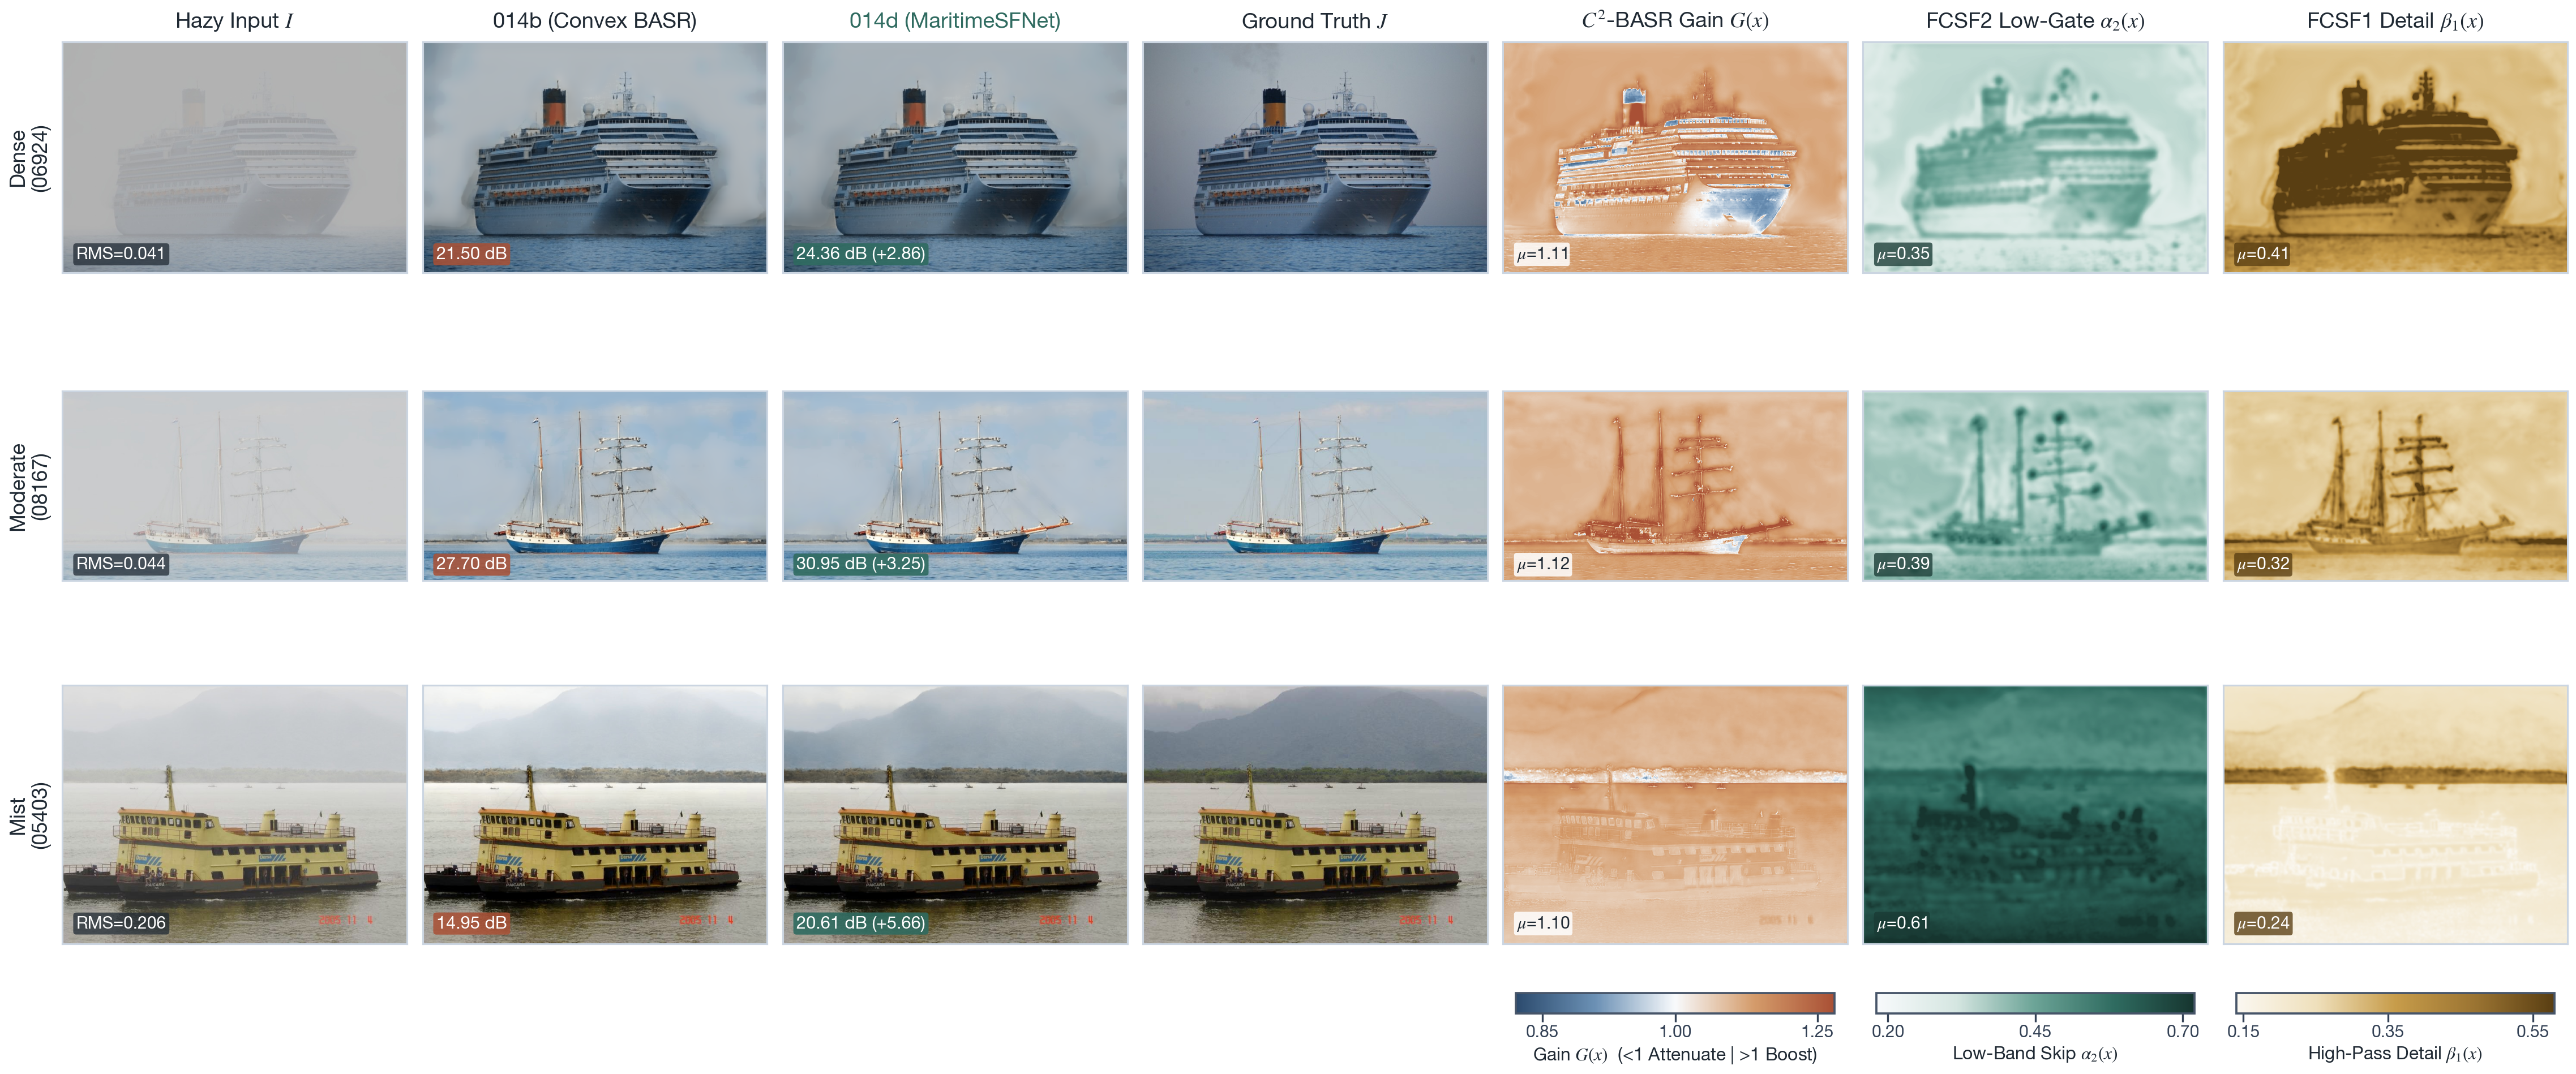
\includegraphics[width=\textwidth]{fig5_spatial_heatmaps.png}
\caption{Visual restoration and internal physical-gate interpretability on three representative OWH maritime scenes spanning Dense (\texttt{06924}, cruise vessel), Moderate (\texttt{08167}, tall sailing ship), and Mist (\texttt{05403}, coastal harbor ferry). Compared with convex-sigmoid \texttt{014b}, \texttt{MaritimeSFNet} (\texttt{014d}) gains $+2.86$\,dB, $+3.25$\,dB, and $+5.66$\,dB while eliminating sky halos and fog veil washout. Columns~5--7 reveal physically meaningful internal behavior: \texttt{$C^2$-BASR} gain $G(x)$ boosts veiled superstructures ($>1.2$, terracotta) while actively attenuating bright highlights and horizon glare ($<1.0$, steel navy); \texttt{FCSF2} low-band gate $\alpha_2(x)$ suppresses hazy low-band passthrough in Dense ($\mu=0.35$) and relaxes in Mist ($\mu=0.61$); \texttt{FCSF1} detail gate $\beta_1(x)$ locks tightly onto ship hulls, masts, and distant coastlines.}
\label{fig:spatial}
\end{figure*}

Fig.~\ref{fig:spatial} visualizes restored images alongside the internal per-pixel physical maps of \texttt{014d} on three diverse maritime scenes: a large ocean cruise liner in dense advection fog (\texttt{Dense\_06924}), a rigged sailing vessel in moderate haze (\texttt{Moderate\_08167}), and a harbor ferry under light coastal mist (\texttt{Mist\_05403}). Beyond dramatic PSNR gains over \texttt{014b} ($+2.86$, $+3.25$, and $+5.66$\,dB), the learned internal fields confirm physical interpretability:
\begin{itemize}
    \item \textbf{Bidirectional $C^2$-BASR Gain $G(x)$:} On the dense cruise ship, $G(x)$ strongly amplifies veiled decks and upper haze ($>1.2$) while dipping strictly below $1.0$ (steel-navy regions) along the bright illuminated bow so specular highlights never clip. On the coastal ferry in light mist, $G(x)$ stays gentle near unity ($\mu=1.10$) and attenuates the bright shoreline horizon line directly.
    \item \textbf{Visibility-Aware \texttt{FCSF2} Low-Band Gate $\alpha_2(x)$:} Under dense fog, $\alpha_2(x)$ stays suppressed ($\mu=0.35$) across the hull and horizon to prevent shallow haze leakage; under light mist, it opens broadly ($\mu=0.61$) to preserve natural scene illumination and water color.
    \item \textbf{Vessel-Selective \texttt{FCSF1} Detail Gate $\beta_1(x)$:} Full-resolution high-pass injection locks onto the cruise liner decks ($\mu=0.41$) and sailing-ship masts/rigging ($\mu=0.32$), while quieting on the already crisp mist ferry foreground ($\mu=0.24$) and focusing selectively on the misty distant mountain shoreline.
\end{itemize}

\subsection{Unsupervised Visibility Manifold Disentanglement (\texorpdfstring{\texttt{t-SNE}}{t-SNE} \& \texorpdfstring{\texttt{K-Means}}{K-Means})}
\label{sec:manifold}

\begin{figure*}[t]
\centering
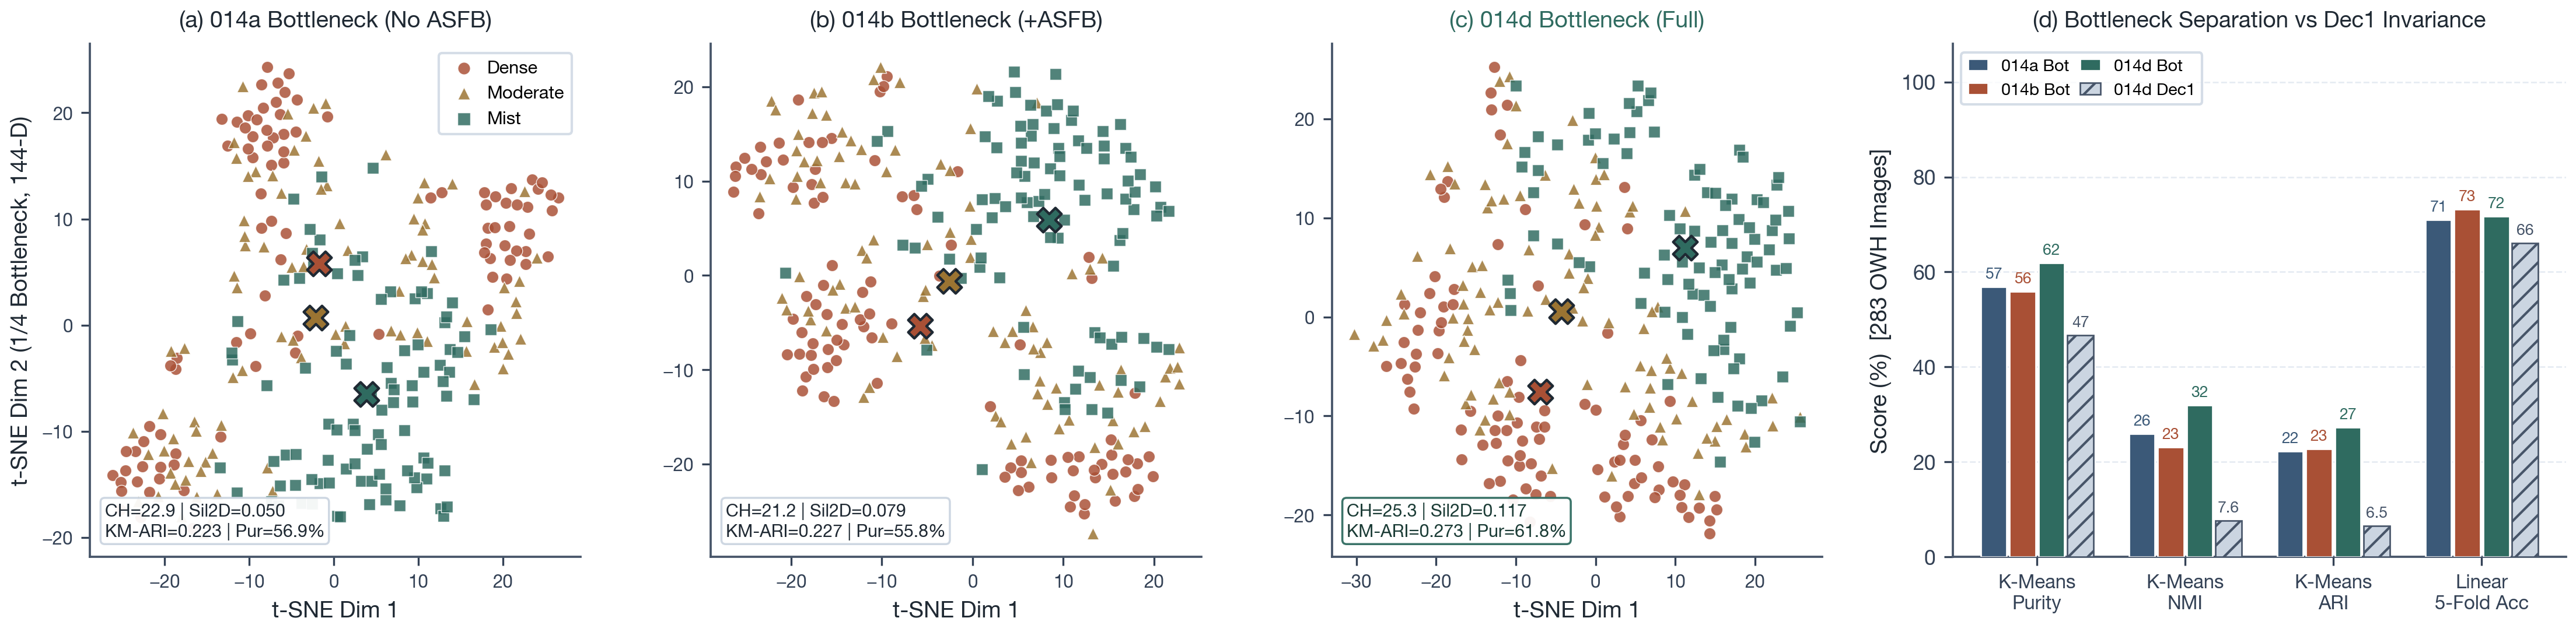
\includegraphics[width=\textwidth]{fig6_tsne_kmeans_visibility.png}
\caption{Train-free feature manifold analysis across all 283 OWH scenes using exact \texttt{t-SNE} and unsupervised \texttt{K-Means++} ($K=3$, 80 restarts) with zero haze-class supervision. \textbf{(a)--(c)}~At the $1/4$ bottleneck ($144$-D), \texttt{014d} forms the sharpest visibility continuum from Dense (terracotta) through Moderate (brass) to Mist (deep teal), boosting Calinski--Harabasz index to $25.3$, K-Means ARI to $0.273$ ($+20.3\%$ vs.\ \texttt{014b}), NMI to $0.319$ ($+38.1\%$), and cluster purity to $61.8\%$. \textbf{(d)}~Stage-wise duality: while \texttt{014d}'s bottleneck maximizes visibility awareness to guide \texttt{MS-LFM}/\texttt{Scene-FCSF}, its pre-BASR decoder (\texttt{014d Dec1}, hatched) deliberately collapses fog-regime separability (NMI $31.9\%\to 7.6\%$, ARI $27.3\%\to 6.5\%$), confirming convergence onto a unified haze-invariant clean scene manifold.}
\label{fig:tsne}
\end{figure*}

A compelling question for restoration interpretability is how the network internally represents sea-fog severity despite receiving \emph{zero} discrete visibility-tier labels during training. We extract global average-pooled feature embeddings from all 283 OWH images at two locations---the $1/4$-scale bottleneck ($144$-D, post-\texttt{ASFB}) and the pre-reconstruction full-resolution decoder \texttt{Dec1} ($36$-D)---and apply exact \texttt{t-SNE} visualization alongside unsupervised \texttt{K-Means++} clustering ($K=3$, 80 restarts, standardized features) and 5-fold linear probing.

\begin{table}[t]
\centering
\caption{Unsupervised \texttt{K-Means++} ($K{=}3$) Visibility Disentanglement at Bottleneck ($144$-D) vs.\ Haze-Invariant Convergence at \texttt{Dec1} ($36$-D)}
\label{tab:manifold}
\renewcommand{\arraystretch}{1.15}
\setlength{\tabcolsep}{3.8pt}
\begin{tabular}{@{}llccccc@{}}
\toprule
\textbf{Feature Stage} & \textbf{Model} & \textbf{CH}$\uparrow$ & \textbf{Sil$_{2\mathrm{D}}$}$\uparrow$ & \textbf{ARI}$\uparrow$ & \textbf{NMI}$\uparrow$ & \textbf{Purity}$\uparrow$ \\
\midrule
\multirow{3}{*}{$1/4$ Bottleneck} & \texttt{014a} & 22.95 & 0.050 & 0.223 & 0.259 & 56.9\% \\
 & \texttt{014b} & 21.17 & 0.079 & 0.227 & 0.231 & 55.8\% \\
 & \textbf{\texttt{014d}} & \textbf{25.26} & \textbf{0.117} & \textbf{0.273} & \textbf{0.319} & \textbf{61.8\%} \\
\midrule
Pre-BASR \texttt{Dec1} & \texttt{014d} & 11.24 & 0.011 & 0.065 & 0.076 & 46.6\% \\
\bottomrule
\end{tabular}
\end{table}

Table~\ref{tab:manifold} and Fig.~\ref{fig:tsne} expose a striking \textbf{encode-disentangle / decode-converge duality}:
\begin{enumerate}
    \item \textbf{Visibility Disentanglement at the Bottleneck:} Even without visibility supervision, \texttt{014d}'s bottleneck separates Dense, Moderate, and Mist along a smooth physical continuum, lifting unsupervised \texttt{K-Means} ARI by \textbf{+20.3\%} ($0.273$ vs.\ $0.227$), NMI by \textbf{+38.1\%} ($0.319$ vs.\ $0.231$), cluster purity by \textbf{+6.0\,pp} ($61.8\%$ vs.\ $55.8\%$), Calinski--Harabasz score by \textbf{+19.3\%} ($25.26$ vs.\ $21.17$), and 2D \texttt{t-SNE} silhouette by \textbf{+135\%} over \texttt{014a} ($0.117$ vs.\ $0.050$). This structured visibility latent directly explains why \texttt{MS-LFM} and \texttt{Scene-FCSF} modulate haze intensity accurately across weather regimes.
    \item \textbf{Haze-Invariant Collapse at \texttt{Dec1}:} By the end of the decoder (\texttt{Dec1}), visibility-tier separability drops sharply (CH $25.26\to 11.24$, NMI $0.319\to 0.076$, ARI $0.273\to 0.065$), confirming that the decoder removes fog-density variation and aligns all three weather tiers onto a single clean-radiance manifold.
\end{enumerate}

\subsection{Lossless Structural Folding and Onboard Real-Time Inference}
\label{sec:folding}

\begin{table}[t]
\centering
\caption{Lossless \texttt{Rep5-CD} Folding Verification and FP32 Inference Throughput on a Single NVIDIA RTX~3090}
\label{tab:folding}
\renewcommand{\arraystretch}{1.15}
\setlength{\tabcolsep}{3.8pt}
\resizebox{\columnwidth}{!}{%
\begin{tabular}{@{}lcccc@{}}
\toprule
\textbf{State} & \textbf{Params} & \textbf{Max Fold Err} & \textbf{$512{\times}512$ (FPS)} & \textbf{720p (FPS)} \\
\midrule
Unfolded (Train) & 7.838M & --- & 38.45\,ms (26.00) & 151.95\,ms (6.58) \\
\textbf{Folded (Deploy)} & \textbf{4.555M} & \textbf{0.00e+00} & \textbf{37.68\,ms (26.54)} & \textbf{151.01\,ms (6.62)} \\
\bottomrule
\end{tabular}}
\end{table}

Table~\ref{tab:folding} confirms exact deployment folding via \texttt{fold\_reparam()}: merging all five \texttt{Rep5-CD} training branches reduces total model size by \textbf{41.89\%} ($7.838\text{M}\to 4.555\text{M}$) with \textbf{bit-exact numerical equivalence} ($\max|\hat{J}_{\mathrm{fold}}-\hat{J}_{\mathrm{train}}|=0.00\times 10^0$ in FP32). At $512\times 512$ input resolution, folded MaritimeSFNet sustains \textbf{26.54\,FPS} ($37.68$\,ms/frame) in standard FP32 without TensorRT or FP16 quantization, and $6.62$\,FPS at $720\text{p}$ ($2.72$\,FPS at $1080\text{p}$), comfortably supporting real-time marine navigation video pipelines.

% =============================================================================
\section{Summary of Design Story}
\label{sec:conclusion}
% =============================================================================

MaritimeSFNet transforms sea-fog restoration from generic backbone scaling into a closed physical-to-architectural chain tailored for maritime perception: empirical sea-fog spectral concentration ($86\%\text{--}87\%$ in $\text{DC}\text{--}0.02$) dictates a three-scale $s=4$ bottleneck via Scale--Bandwidth Alignment; horizontal/vertical sea--sky stratification motivates translation-equivariant \texttt{ASFB} and \texttt{L2-AnisoLK} context; mid-band vessel silhouette clarity drives zero-DC \texttt{Rep5-CD} and residual \texttt{DCA-PA}; shallow veil passthrough is blocked by visibility-adaptive convex \texttt{Scene-FCSF}; and Mist-to-Dense dynamic range bias is mathematically eliminated by $C^2$ zero-curvature \texttt{$C^2$-BASR} with RMS-contrast scene gating. Every theoretical property is independently corroborated by train-free spectral, ERF, gate-map, and feature-manifold experiments, providing both a strong synthetic restoration backbone and a cleanly decoupled four-interface anchor for real-world maritime domain adaptation.

\balance
\end{document}
